\section{Dijet Monte Carlo Studies} %updated June 16 2017
\label{app:dijetMC_studies}

%%\paragraph{}
The kinematic variables used for reweighting the data (Section~\ref{sec:boosted-reweight}) have been also studied in dijet monte carlo (MC), and they are presented in this section. By comparing the relevant distributions in both the MC and the data, we would like to understand if the shape discrepancy between the data regions which have different number of b-tagged track jet multiplicity, can also be observed in MC or not. If such an effect exists and its behaviour has a same trend with data, it can support the argument that b-tagging is sculpting the distributions. In this case, it is clear that those variables must be reweighted both in data and MC in order to obtain correct background estimation by compensating the artefact coming from b-tagging.

%%\paragraph{}
6 variables have been studied seperately; 2 of them are $p_{T}$'s of the Higgs candidates and the other 4 are $p_{T}$'s of the first two leading track jets in each Higgs candidates. Distributions are checked in the extended 2bs sideband region of the dijet MC, where the sideband radius is increased up to 1 TeV in order to enrich the statistics.  0 Tag region (0b) and 2 Tag split region (2bs) are used as they are and 1 Tag region is splitted into 2 orthogonal regions according to the position of the b-tagged track jet; if the b-tagged track jet is on the leading Higgs candidate (1bL) or on the subleading Higgs candidate (1bSL). 4 track jet distributions have been shown in Figure~\ref{fig:TjMC} and it is possible to infer the following statements.

\begin{itemize}
\item Looking at the track jets on the leading Higgs candidate, one can see that 1bSL and 0b are one group behaving similarly to each other, while 1bL and 2bs are another group which has a similar trend with each other but different than the other group. 
\item Looking at the track jets on the subleading Higgs candidate, one can see that 1bL and 0b are one group behaving similarly to each other and 1bSL and 2bs are another group which has a similar trend with each other but different than the other group.
\item Both the leading and the subleading track jet distributions behave same if they belong to the same Higgs candidate. Around 300-350 GeV, different regions coincides with each other and then they change their trends to the opposite direction.
\end{itemize}
 
\begin{figure*}[htbp!]
\begin{center}
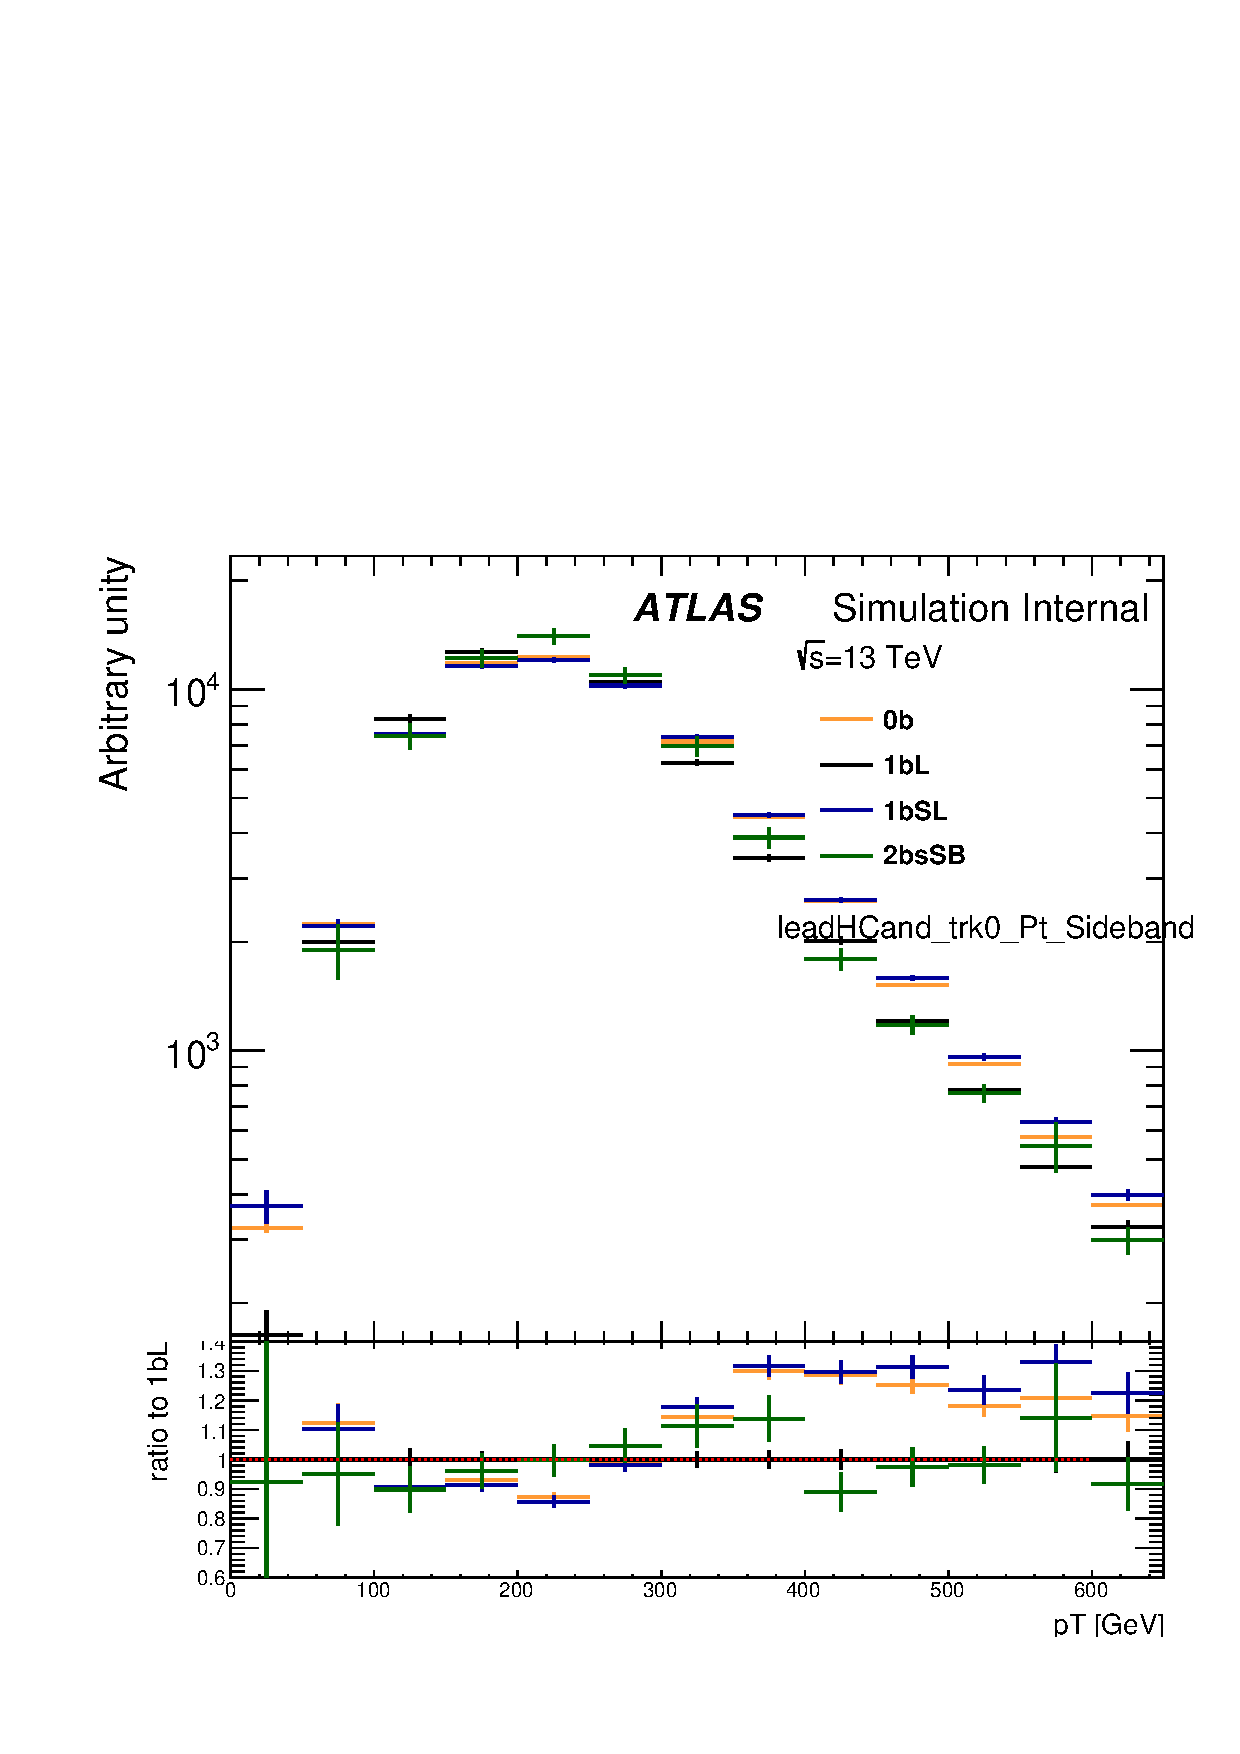
\includegraphics[width=0.45\textwidth,angle=-90]{figures/boosted/AppendixDijetMC/leadHCand_trk0_Pt_SidebandwoPr_log.pdf}
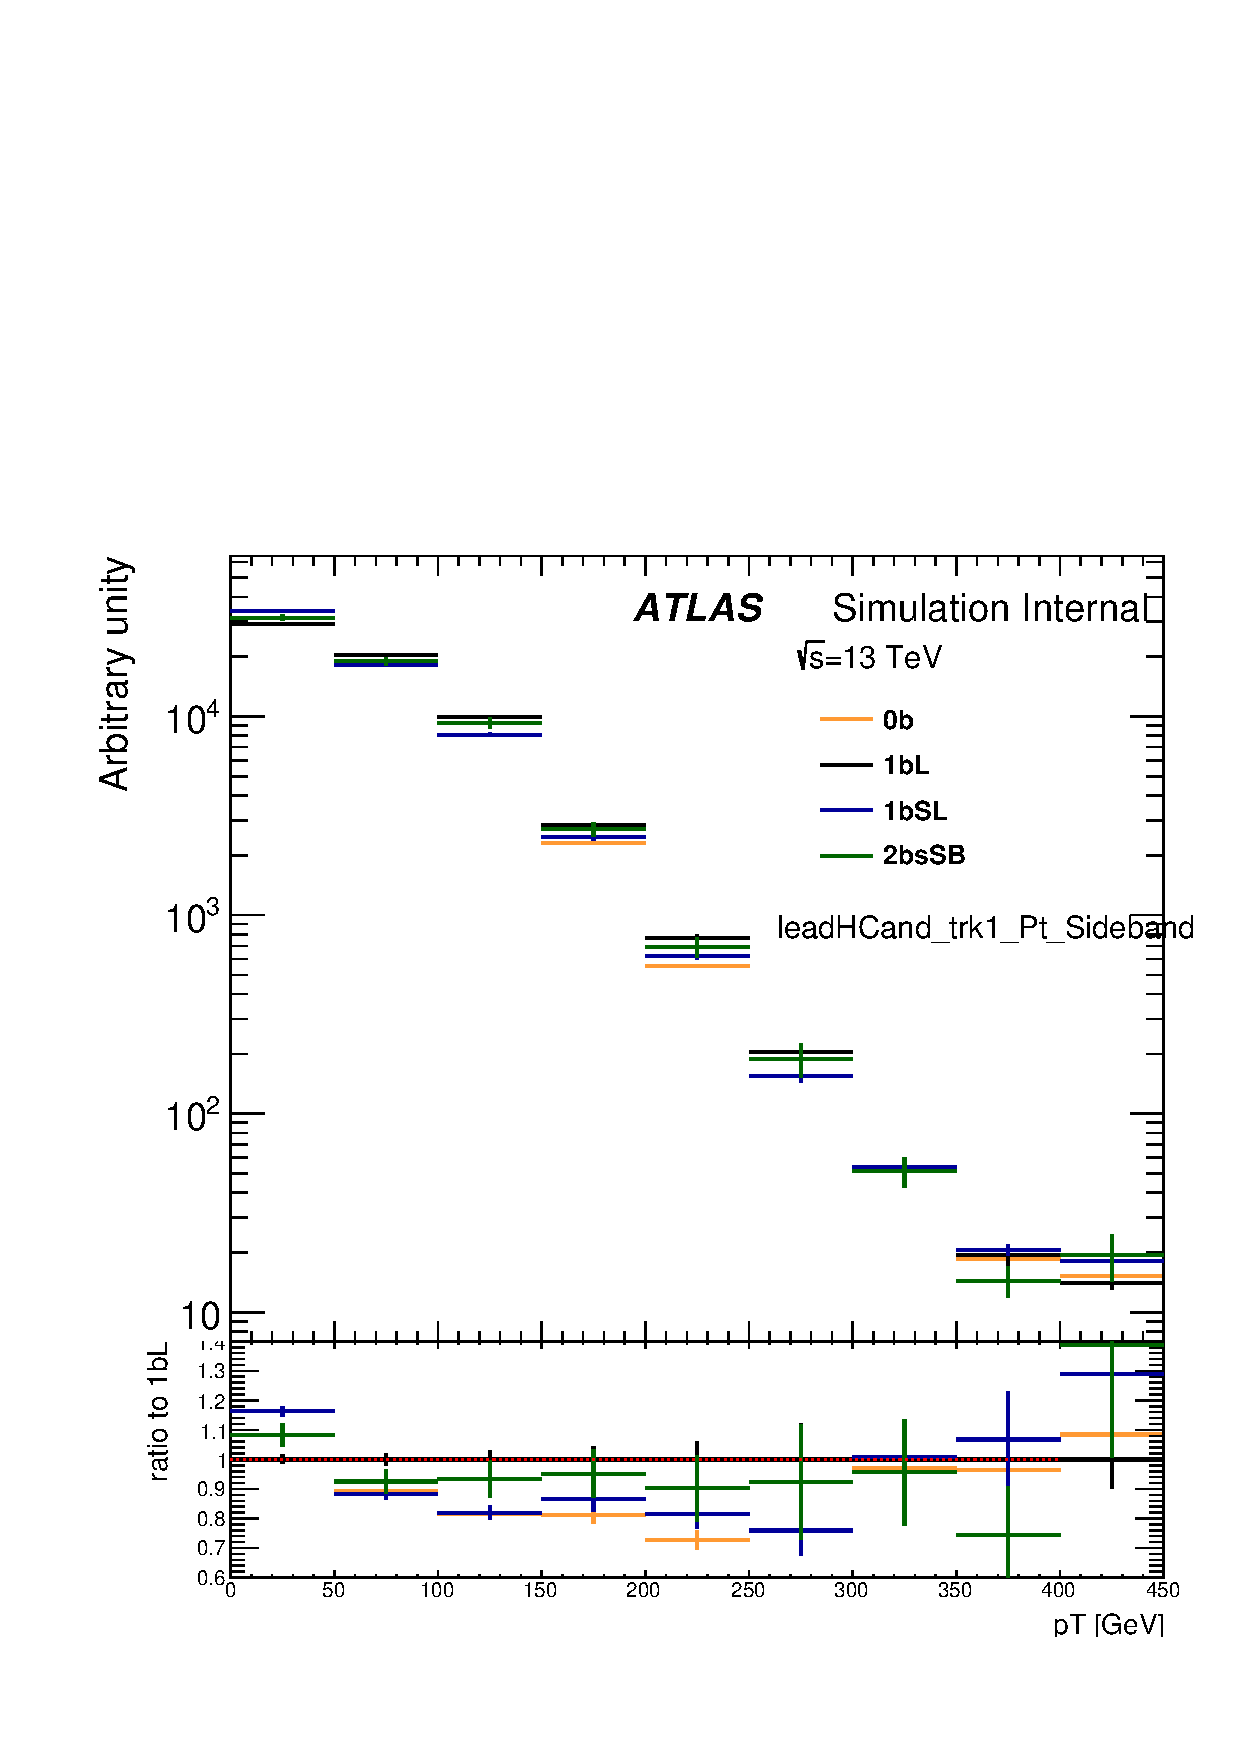
\includegraphics[width=0.45\textwidth,angle=-90]{figures/boosted/AppendixDijetMC/leadHCand_trk1_Pt_SidebandwoPr_log.pdf}
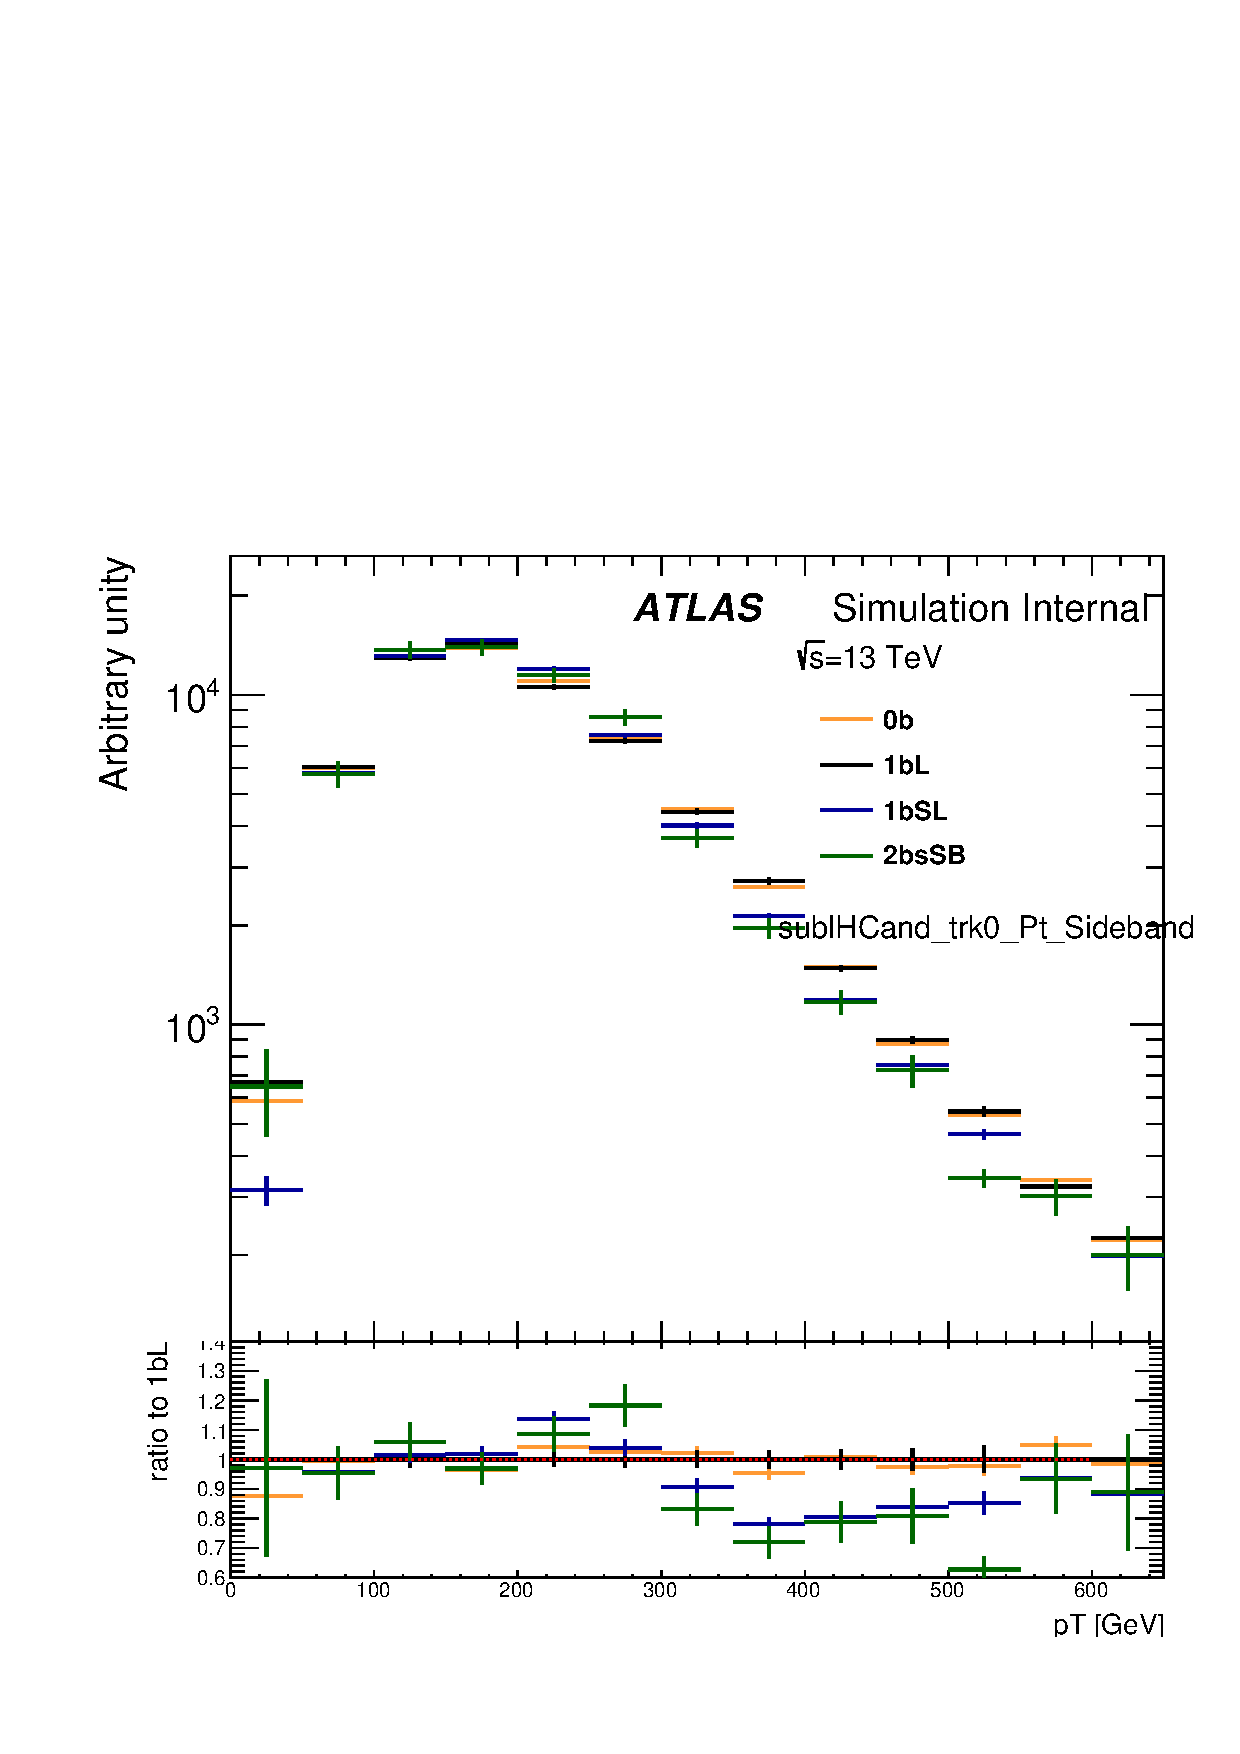
\includegraphics[width=0.45\textwidth,angle=-90]{figures/boosted/AppendixDijetMC/sublHCand_trk0_Pt_SidebandwoPr_log.pdf}
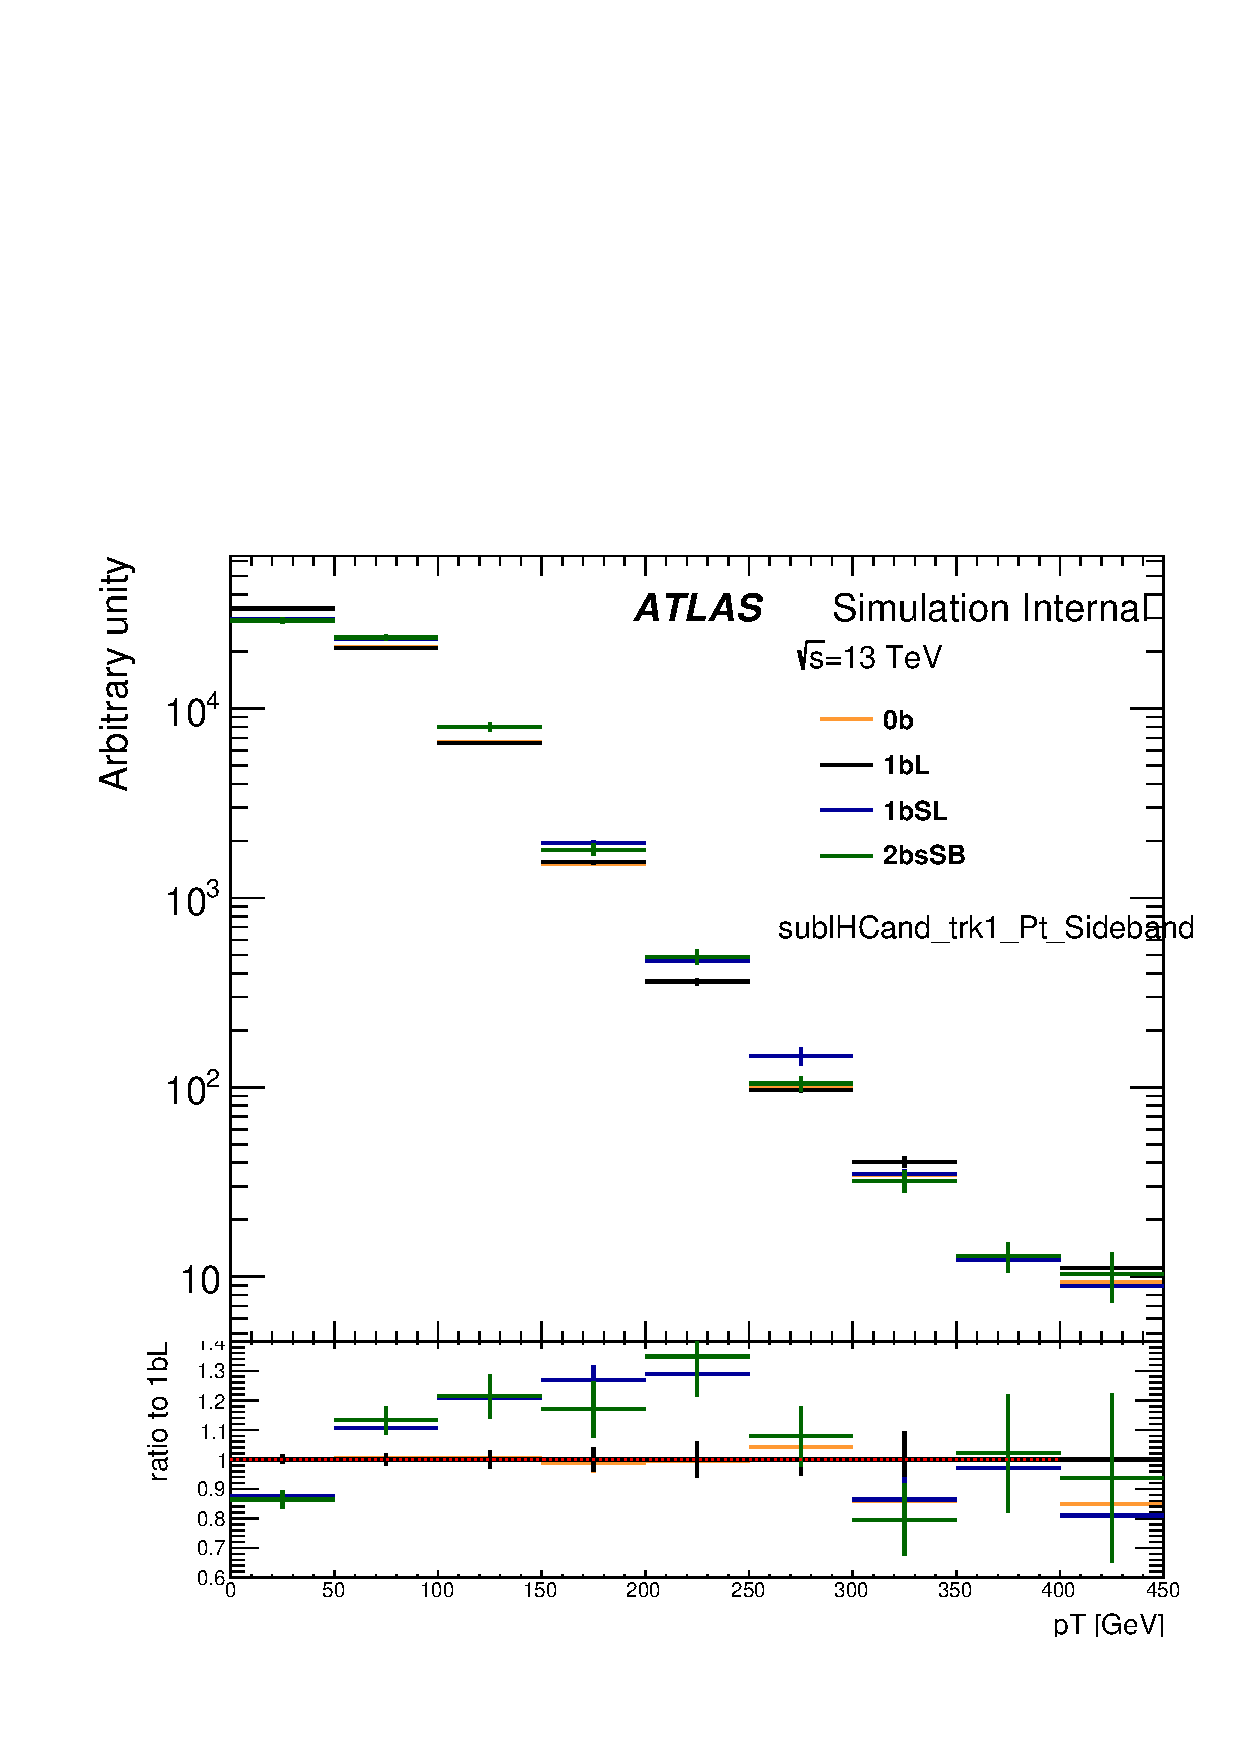
\includegraphics[width=0.45\textwidth,angle=-90]{figures/boosted/AppendixDijetMC/sublHCand_trk1_Pt_SidebandwoPr_log.pdf}
 \caption{Track jet $p_{T}$ distributions in Dijet MC. (Top left) Leading track jet on leading Higgs candidate, (top right) subleading track jet on leading Higgs candidate, (bottom left) leading track jet on subleading Higgs candidate and (bottom right) subleading track jet on subleading Higgs candidate have been shown for the different regions as described in the text. All distributions are normalised according to the 2bs region.}
\label{fig:TjMC}
\end{center}
\end{figure*}

%%\paragraph{}
When the same variables have been plotted in data using the standard sideband region definition, it can be clearly seen that all of the statements above also hold for the distributions in data, as shown in Figure~\ref{fig:TjData}. The amount of the discrepancies are about the same order in both data and MC, only the error bars in data much more smaller because of the higher statistics. 
From those results it is possible to argue that; 
\begin{itemize}
\item$p_{T}$ of the track jets in the subleading Higgs candidate must be reweighted to look like the track jets in the leading Higgs candidate in order to estimate 2bs background from the 1bL region. 
\item$p_{T}$ of the track jets in the leading Higgs candidate must be reweighted to look like the track jets in the subleading Higgs candidate in order to estimate 2bs background from the 1bSL region. 
\end{itemize}  
These results are motivating the AddTag reweighting method, which is described in Section~\ref{sec:boosted-reweight}. 

%%\paragraph{}
Furthermore, the background predictions for the 2bs region before applying any reweighting have been shown in the Figure~\ref{fig:TjPred} for all the track jet $p_{T}$ distributions. The predictions stand between the 0b region and the 2bs regions, as expected from the background modelling method(Section~\ref{sec:backgrounds}). Addition of the 1bL and 1bSL provides a partial recovery for the shape differences between 0b and 2bs regions. However, the predictions still need to be reweighted. As a result of those studies, it has been confirmed that similar reweighting is needed for dijet MC, in a similar manner as data. 

\begin{figure*}[htbp!]
\begin{center}
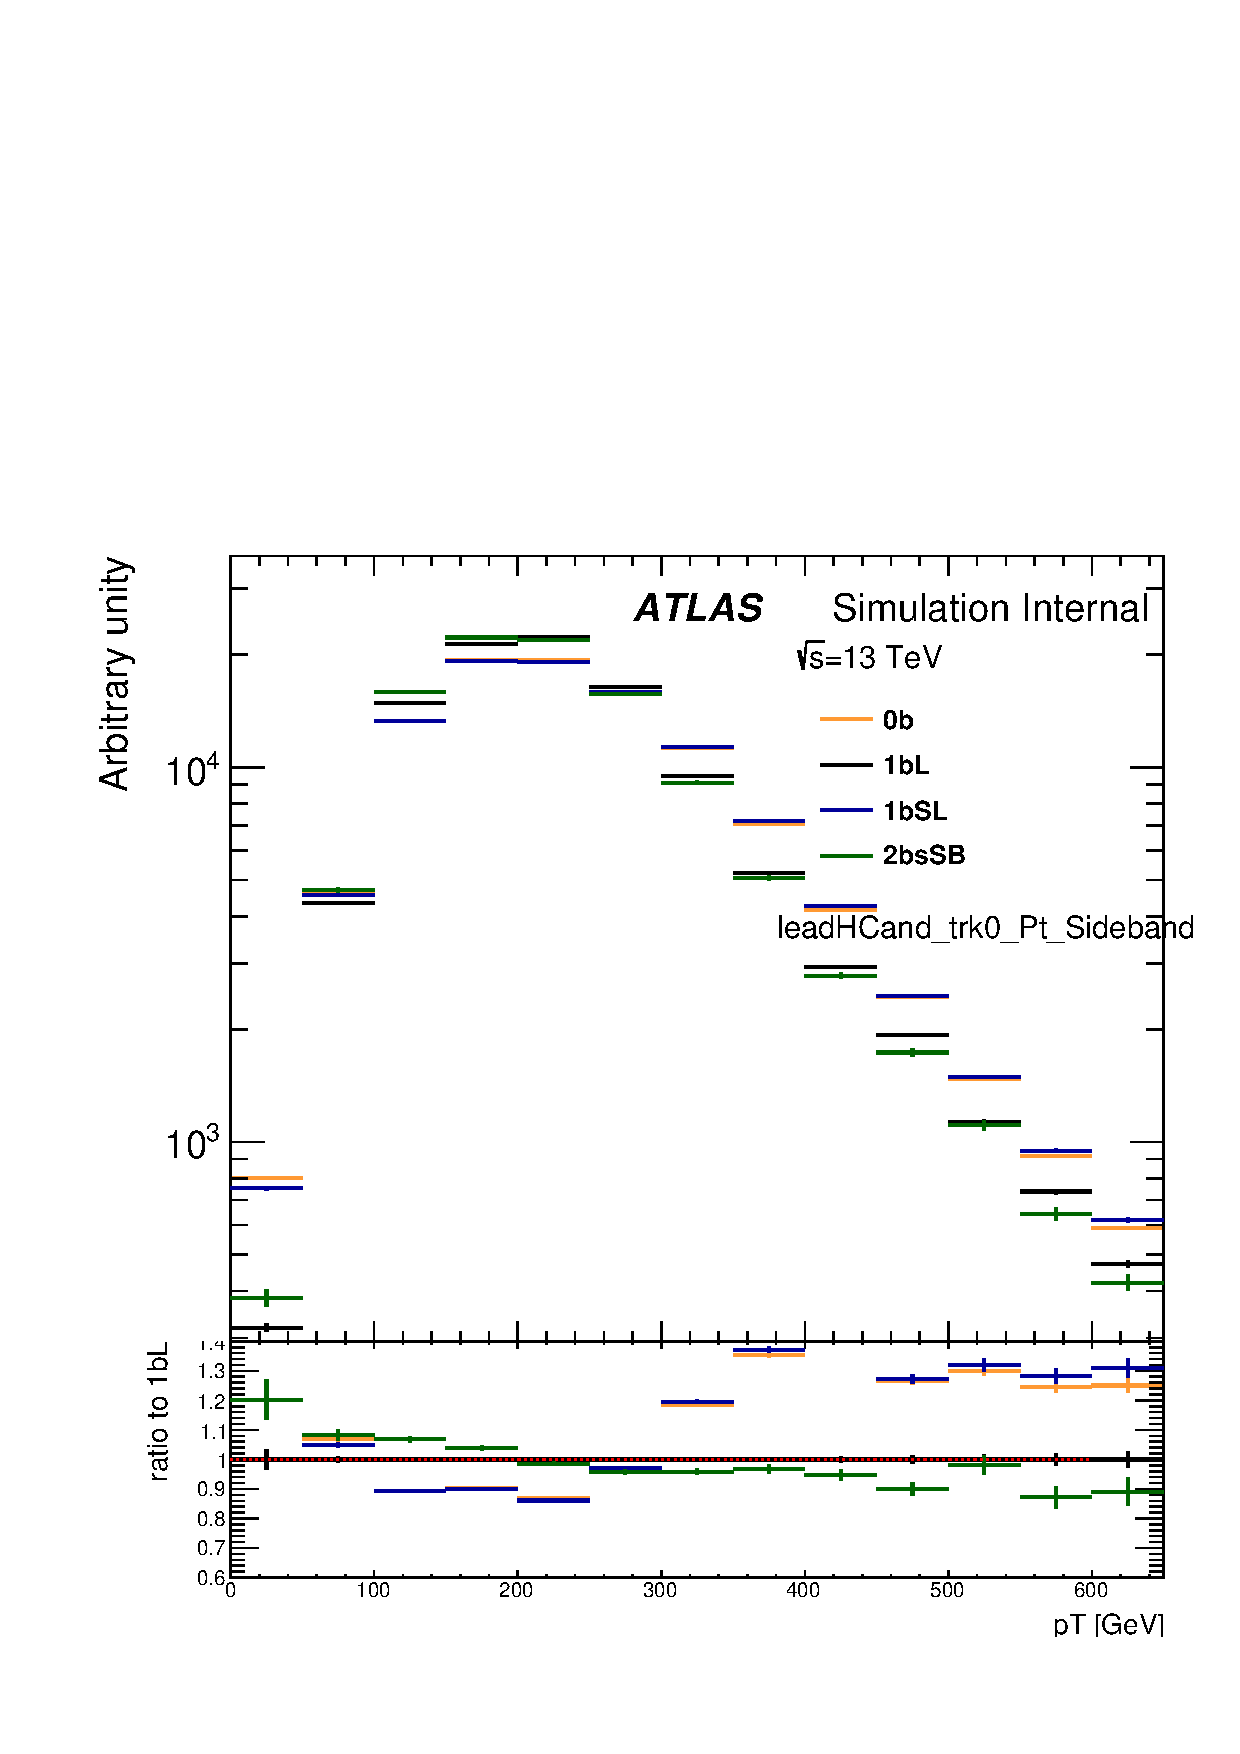
\includegraphics[width=0.45\textwidth,angle=-90]{figures/boosted/AppendixDijetMC/leadHCand_trk0_Pt_SidebandwoPr_data.pdf}
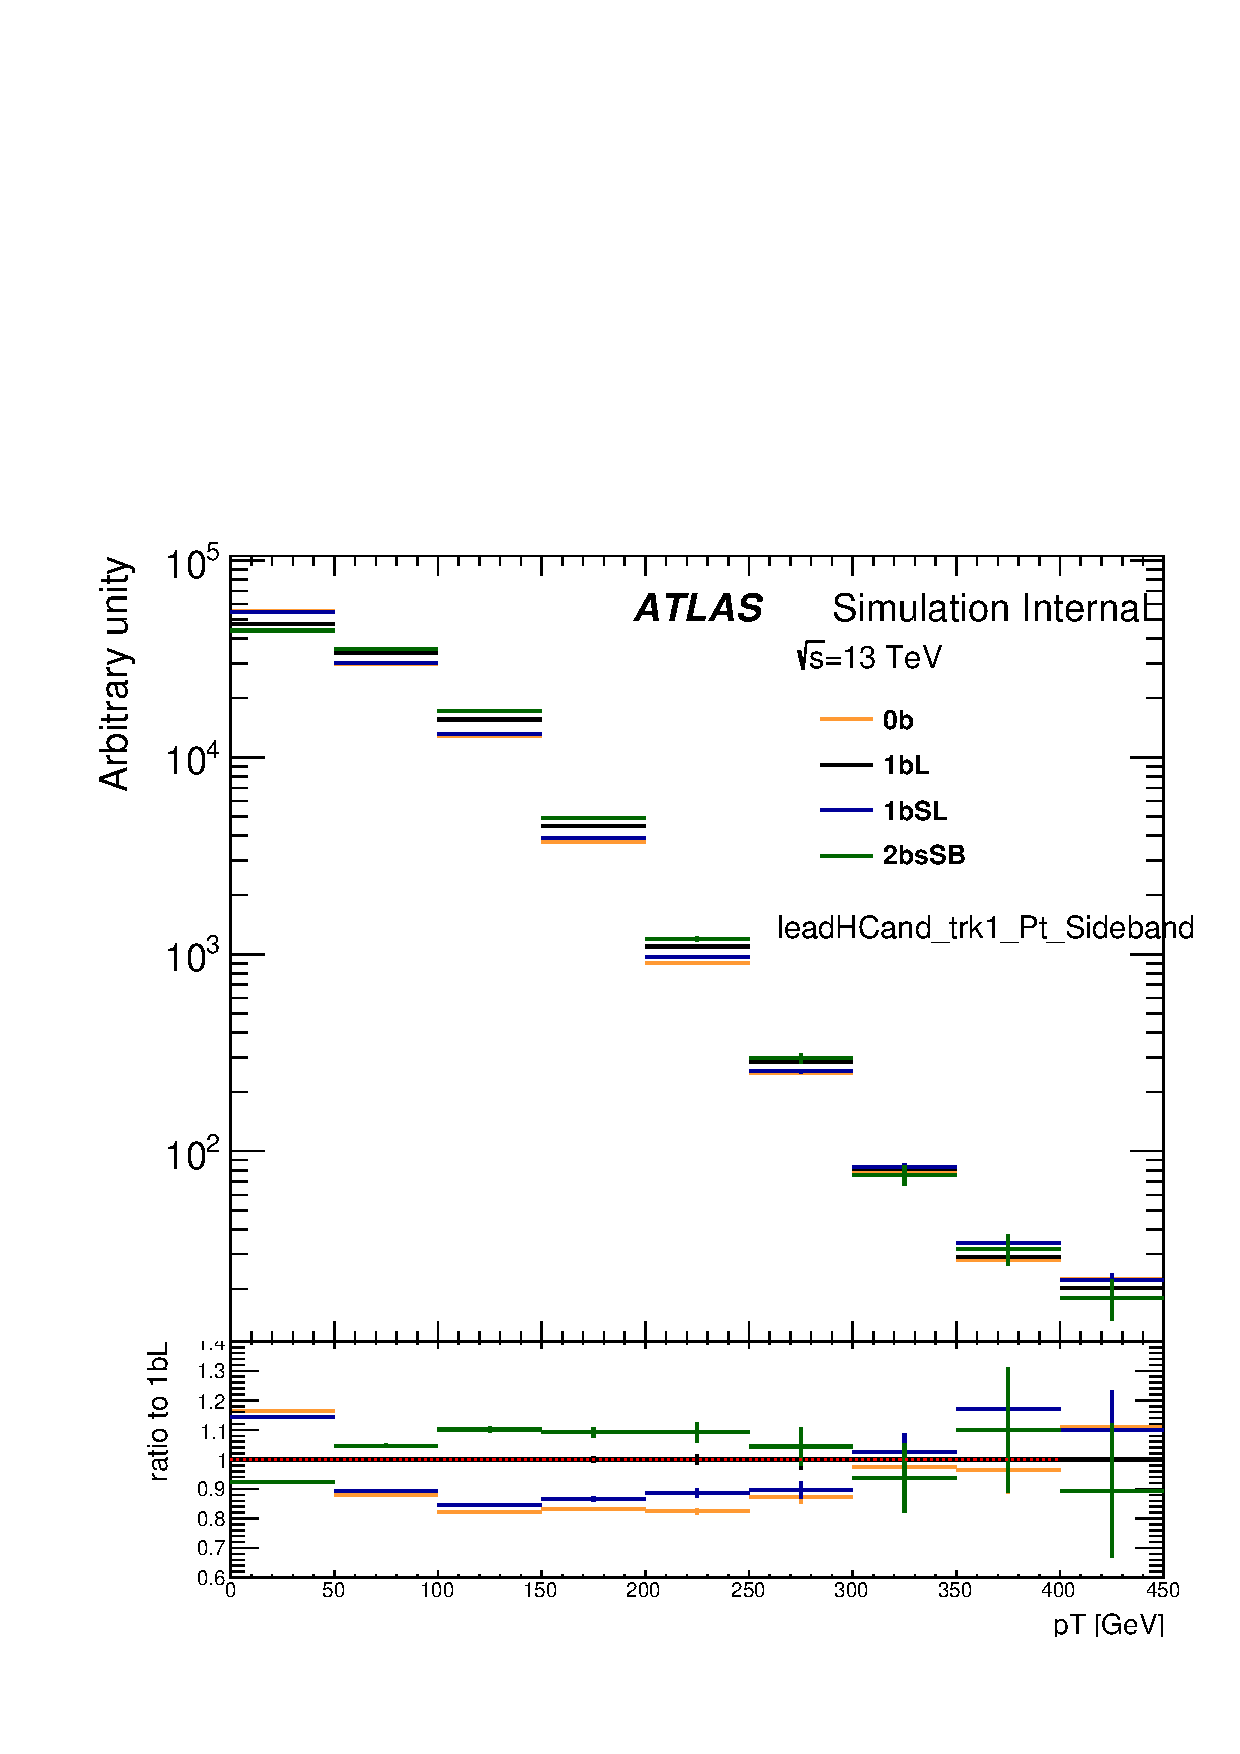
\includegraphics[width=0.45\textwidth,angle=-90]{figures/boosted/AppendixDijetMC/leadHCand_trk1_Pt_SidebandwoPr_data.pdf}
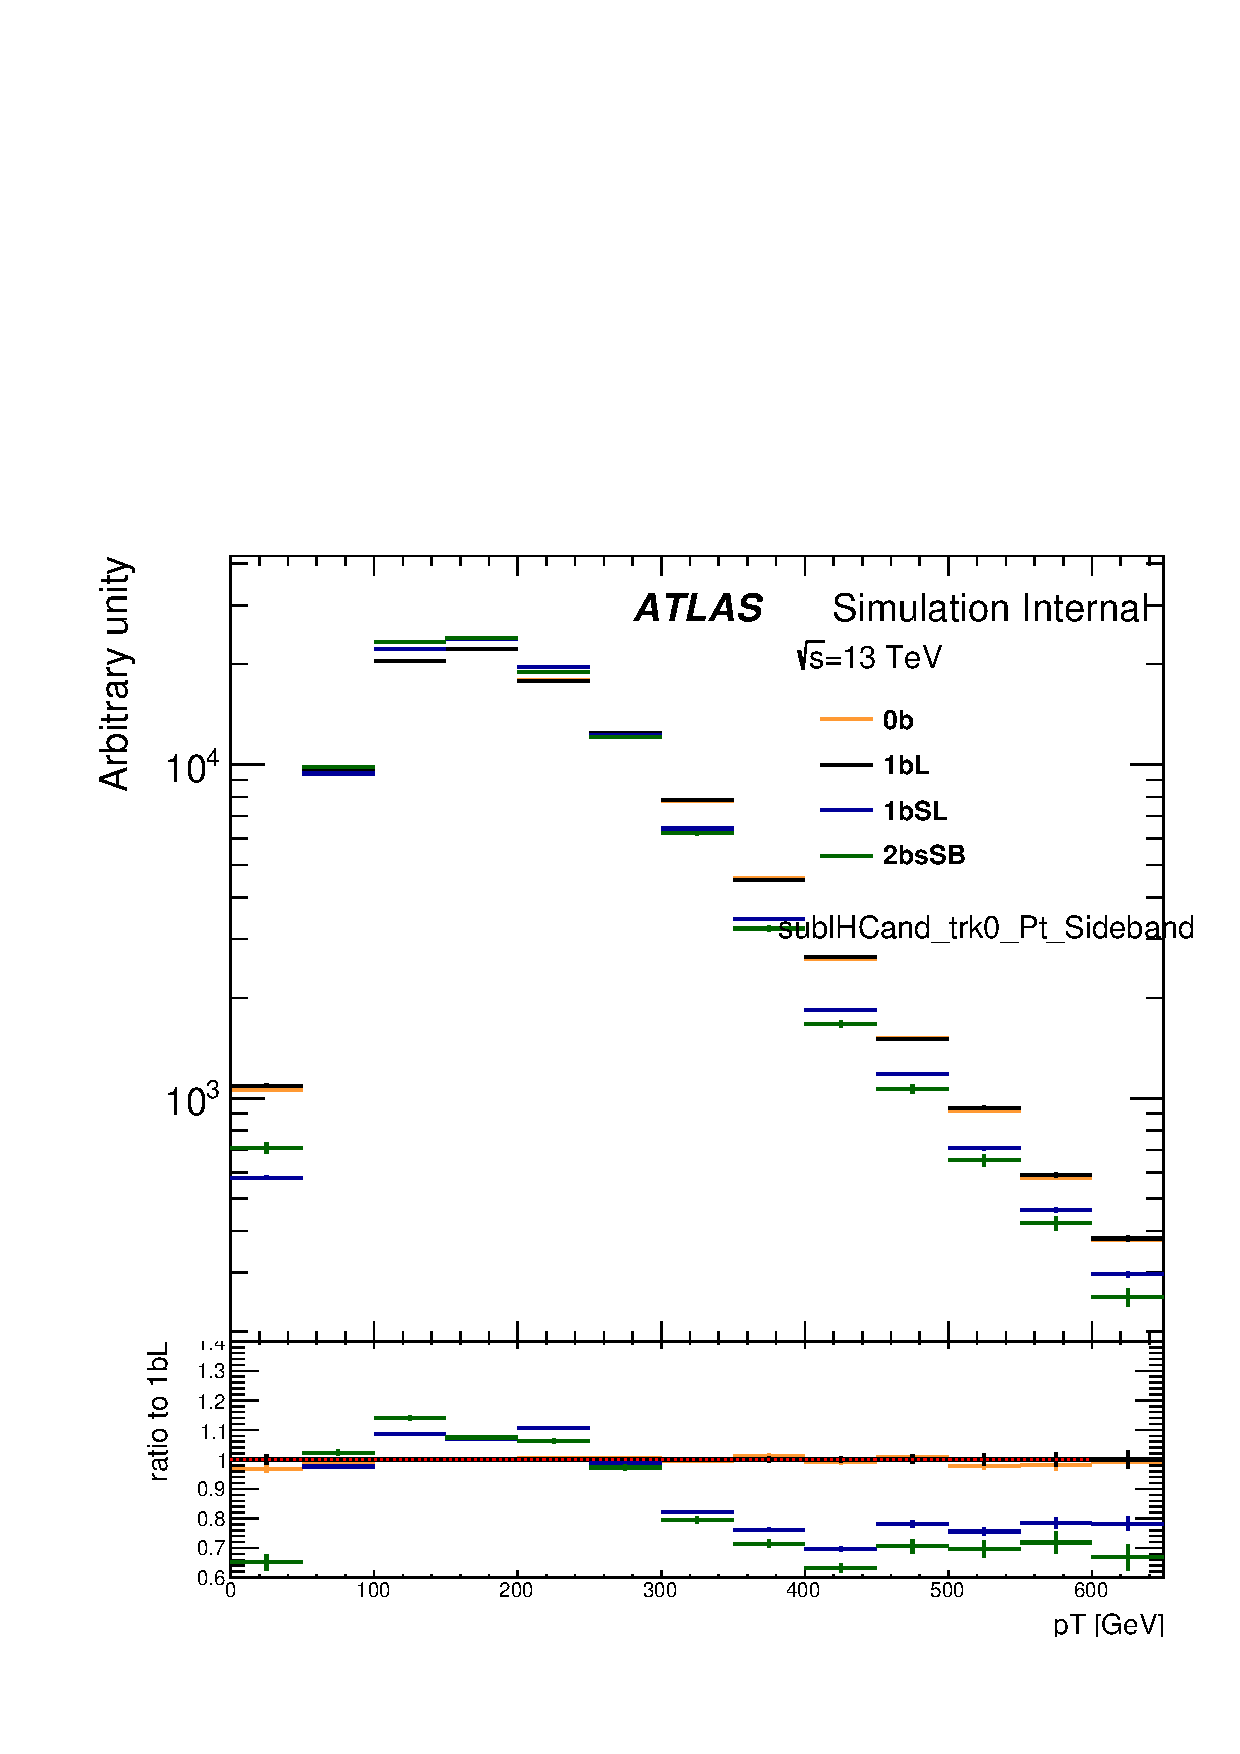
\includegraphics[width=0.45\textwidth,angle=-90]{figures/boosted/AppendixDijetMC/sublHCand_trk0_Pt_SidebandwoPr_data.pdf}
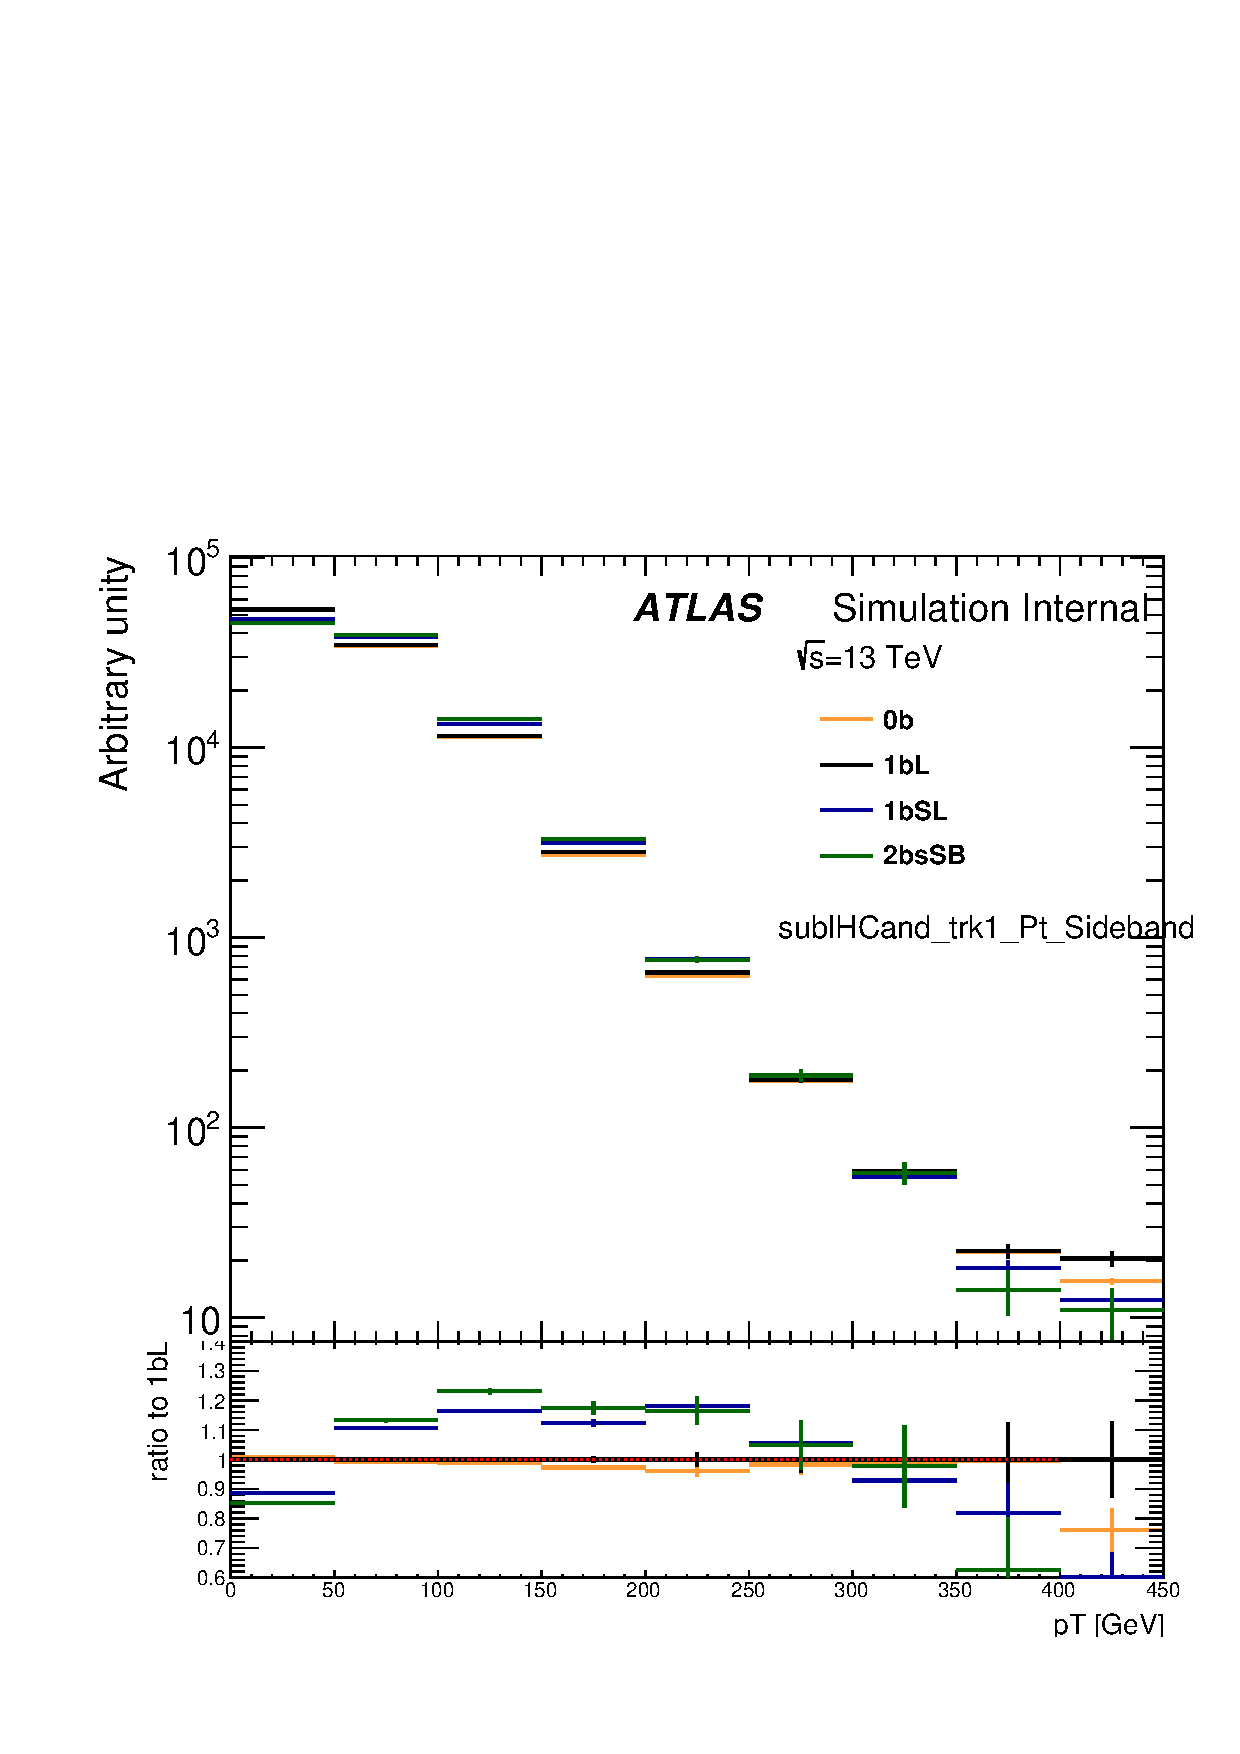
\includegraphics[width=0.45\textwidth,angle=-90]{figures/boosted/AppendixDijetMC/sublHCand_trk1_Pt_SidebandwoPr_data.pdf}

 \caption{Track jet $p_{T}$ distributions in Data. (Top left) Leading track jet on leading Higgs candidate, (top right) subleading track jet on leading Higgs candidate, (bottom left) leading track jet on subleading Higgs candidate and (bottom right) subleading track jet on subleading Higgs candidate have been shown for the different regions as described in the text. All distributions are normalised according to the 2bs region.}

\label{fig:TjData}
\end{center}
\end{figure*}

\begin{figure*}[htbp!]
\begin{center}
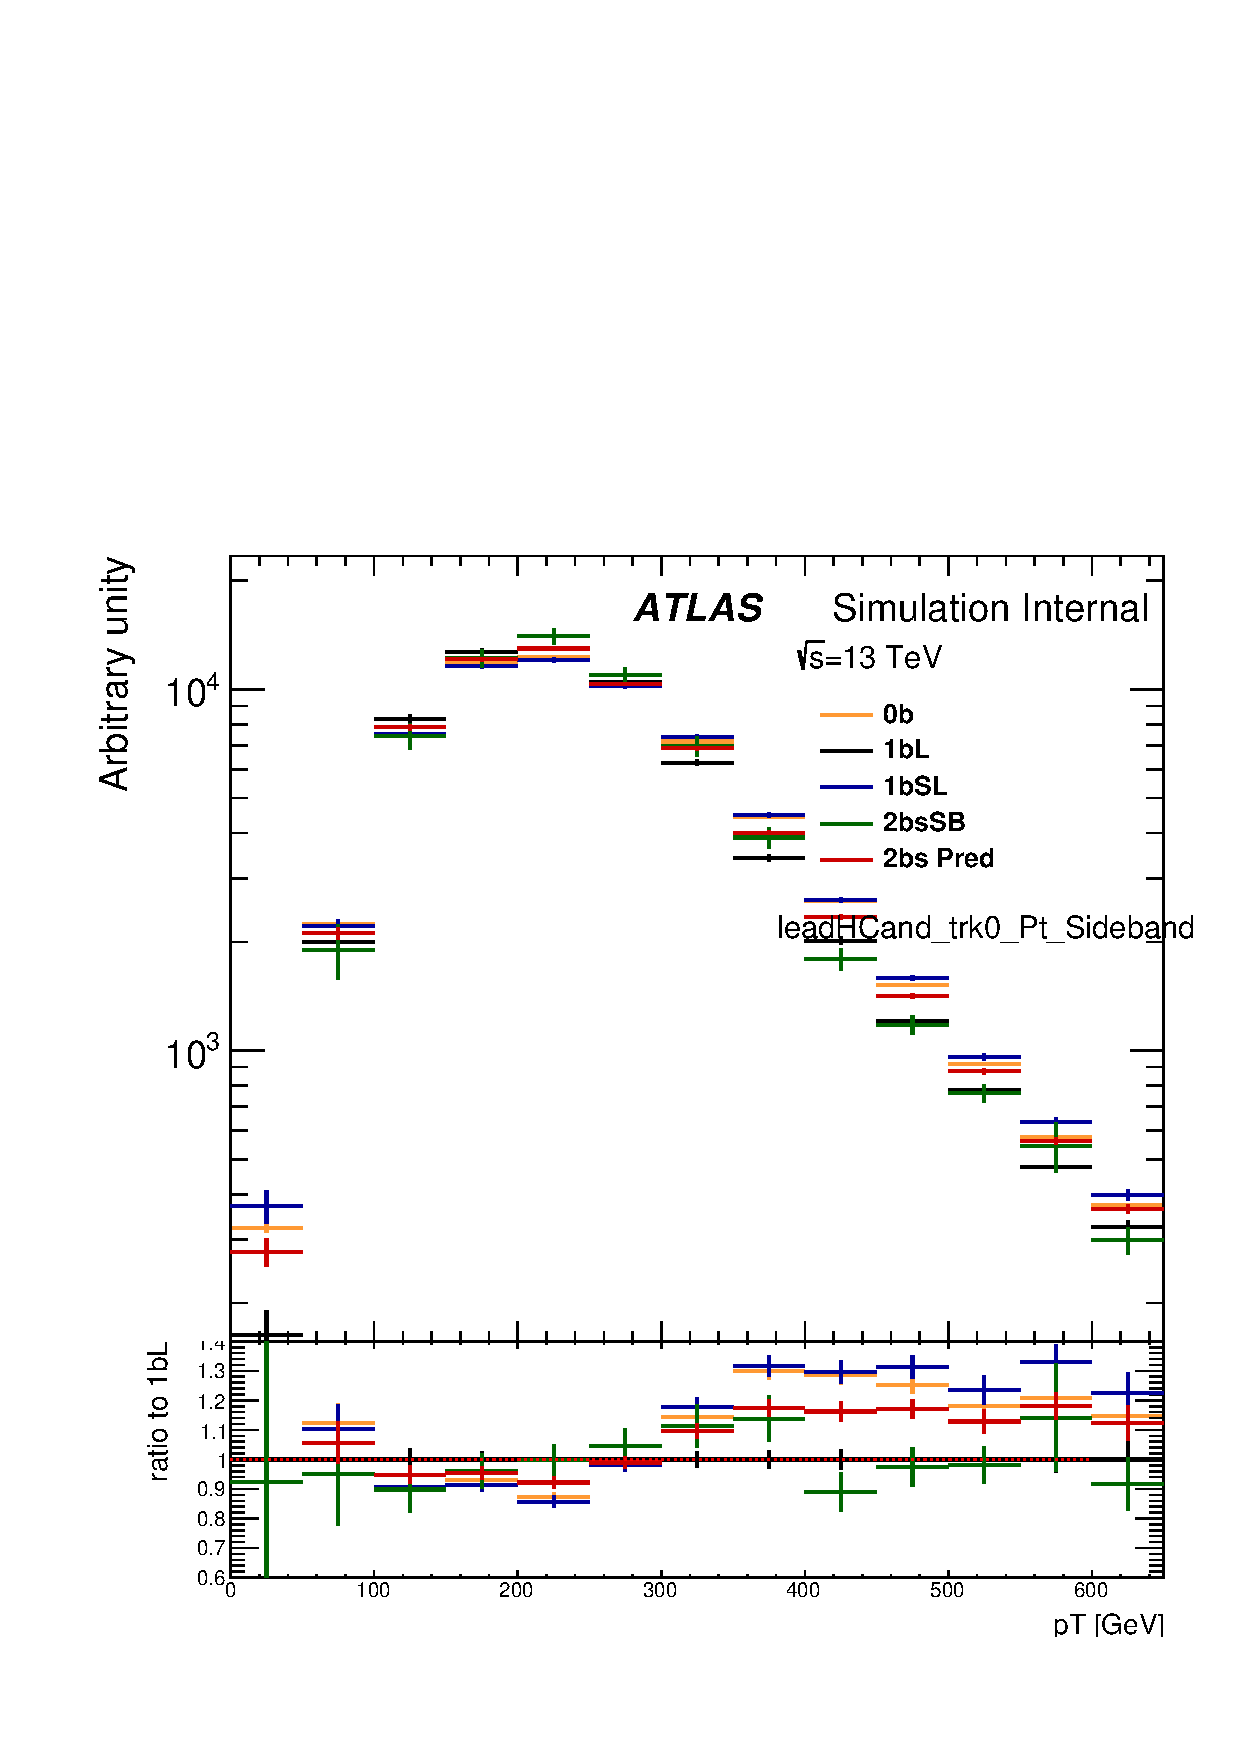
\includegraphics[width=0.25\textwidth,angle=-90]{figures/boosted/AppendixDijetMC/leadHCand_trk0_Pt_Sidebandlessbin_log.pdf}
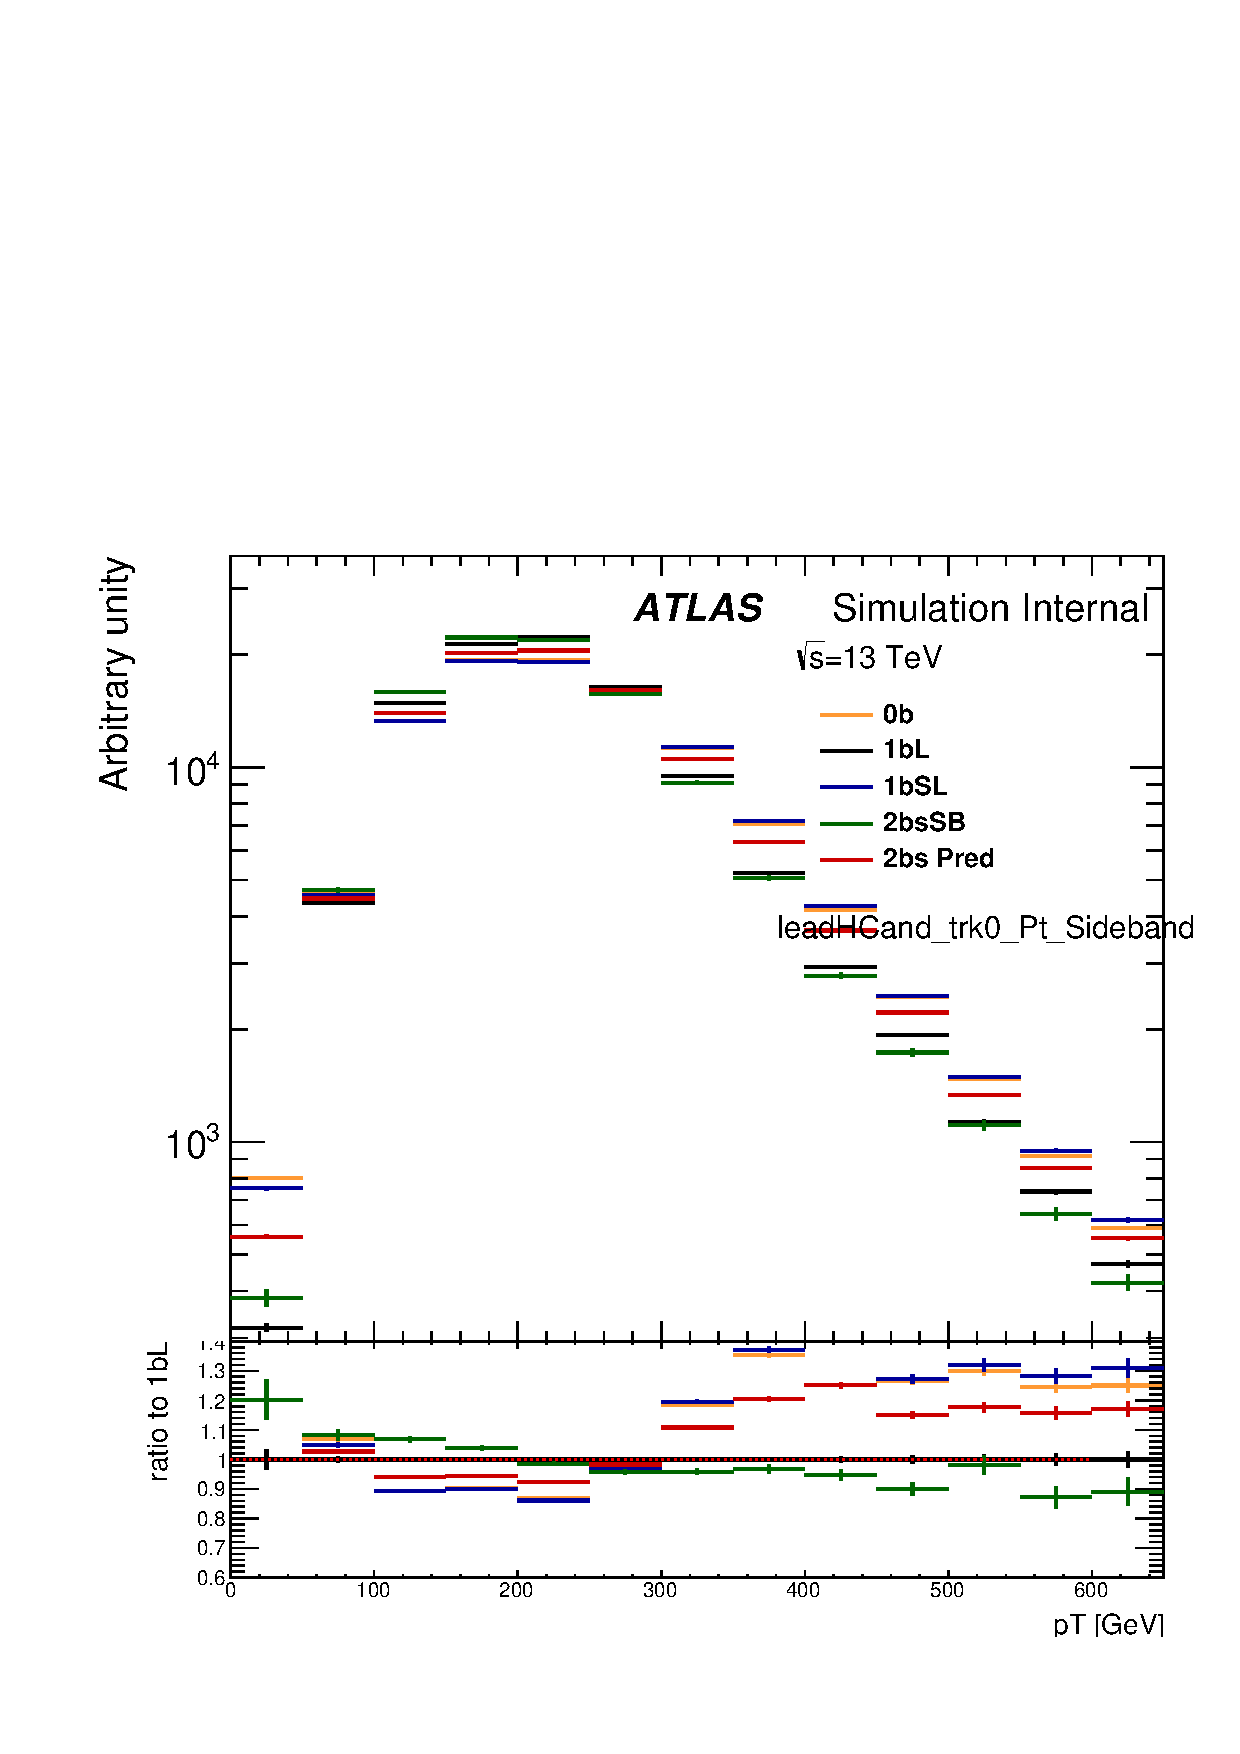
\includegraphics[width=0.25\textwidth,angle=-90]{figures/boosted/AppendixDijetMC/leadHCand_trk0_Pt_Sidebanddata_log.pdf}\\
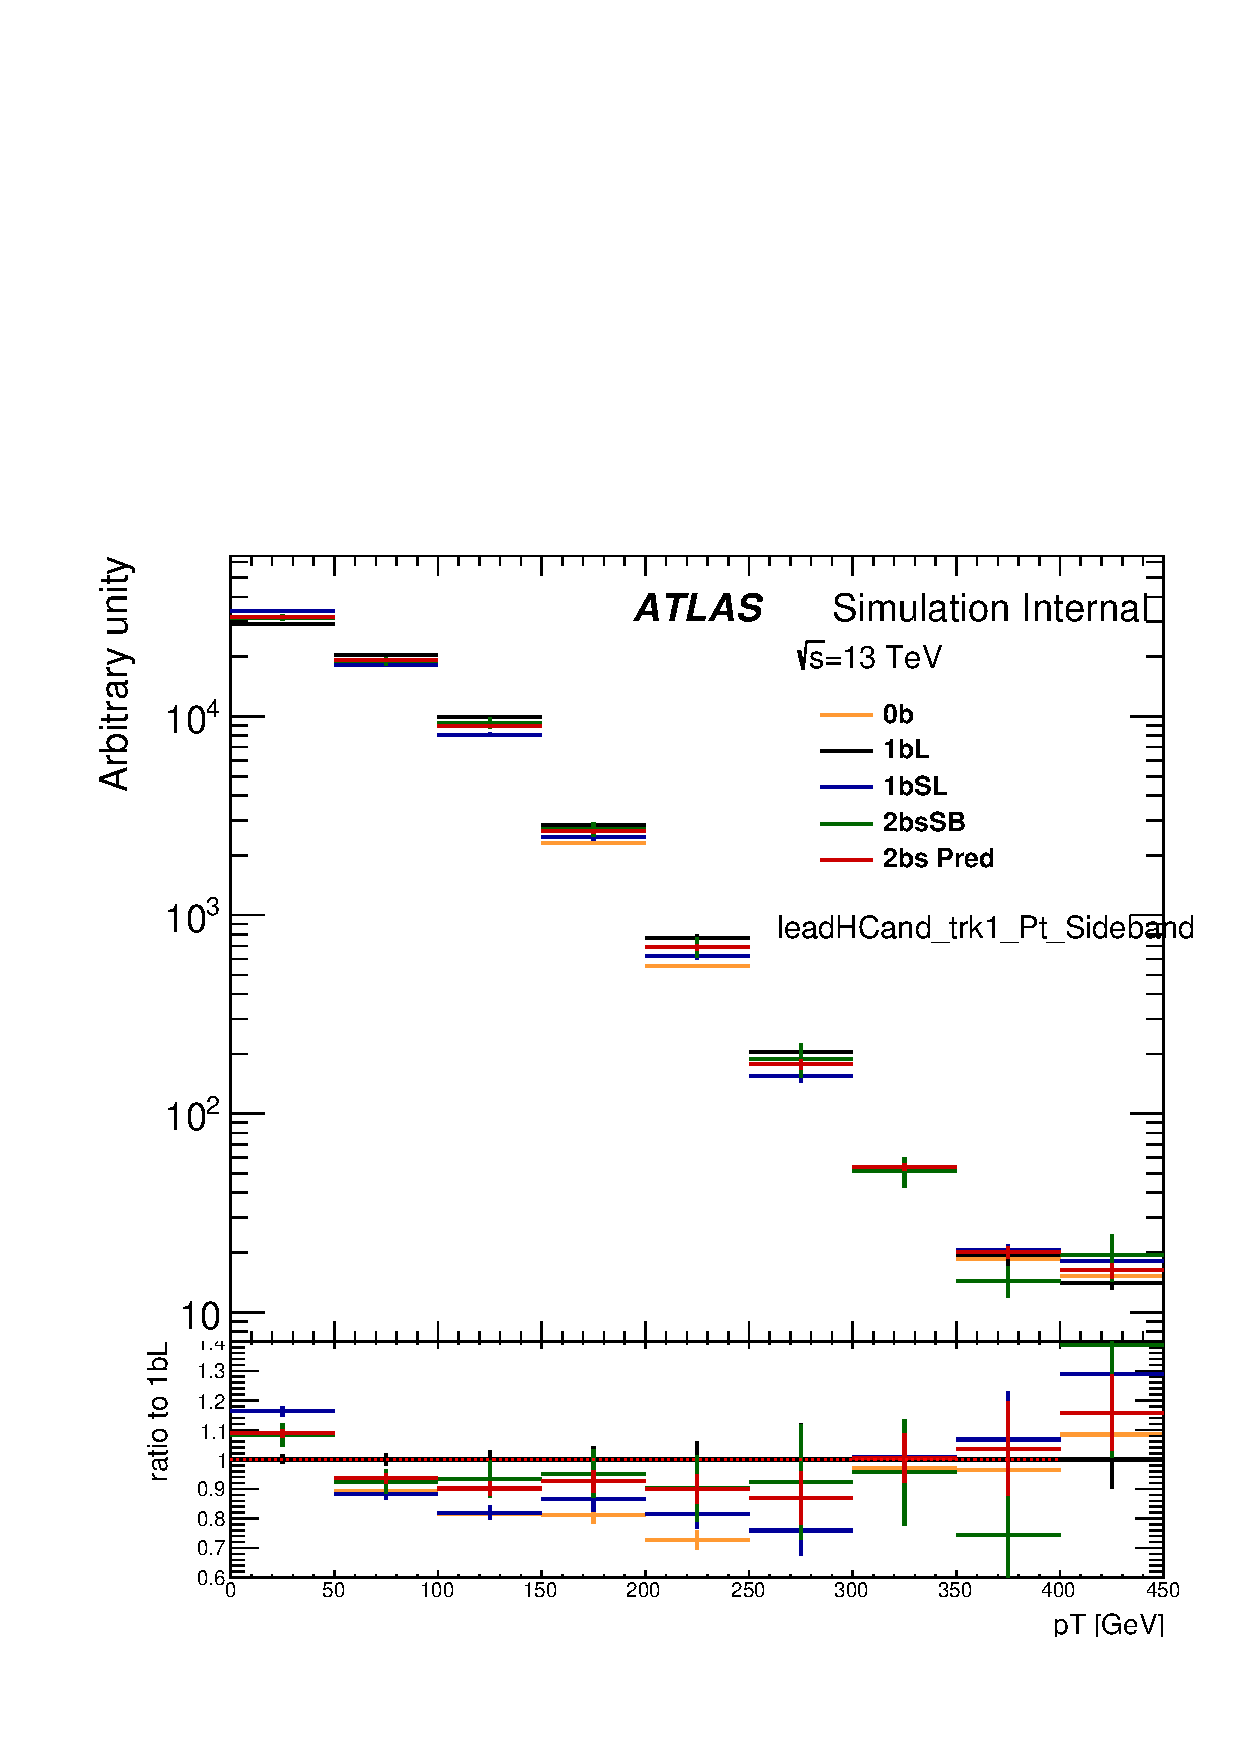
\includegraphics[width=0.25\textwidth,angle=-90]{figures/boosted/AppendixDijetMC/leadHCand_trk1_Pt_Sidebandlessbin_log.pdf}
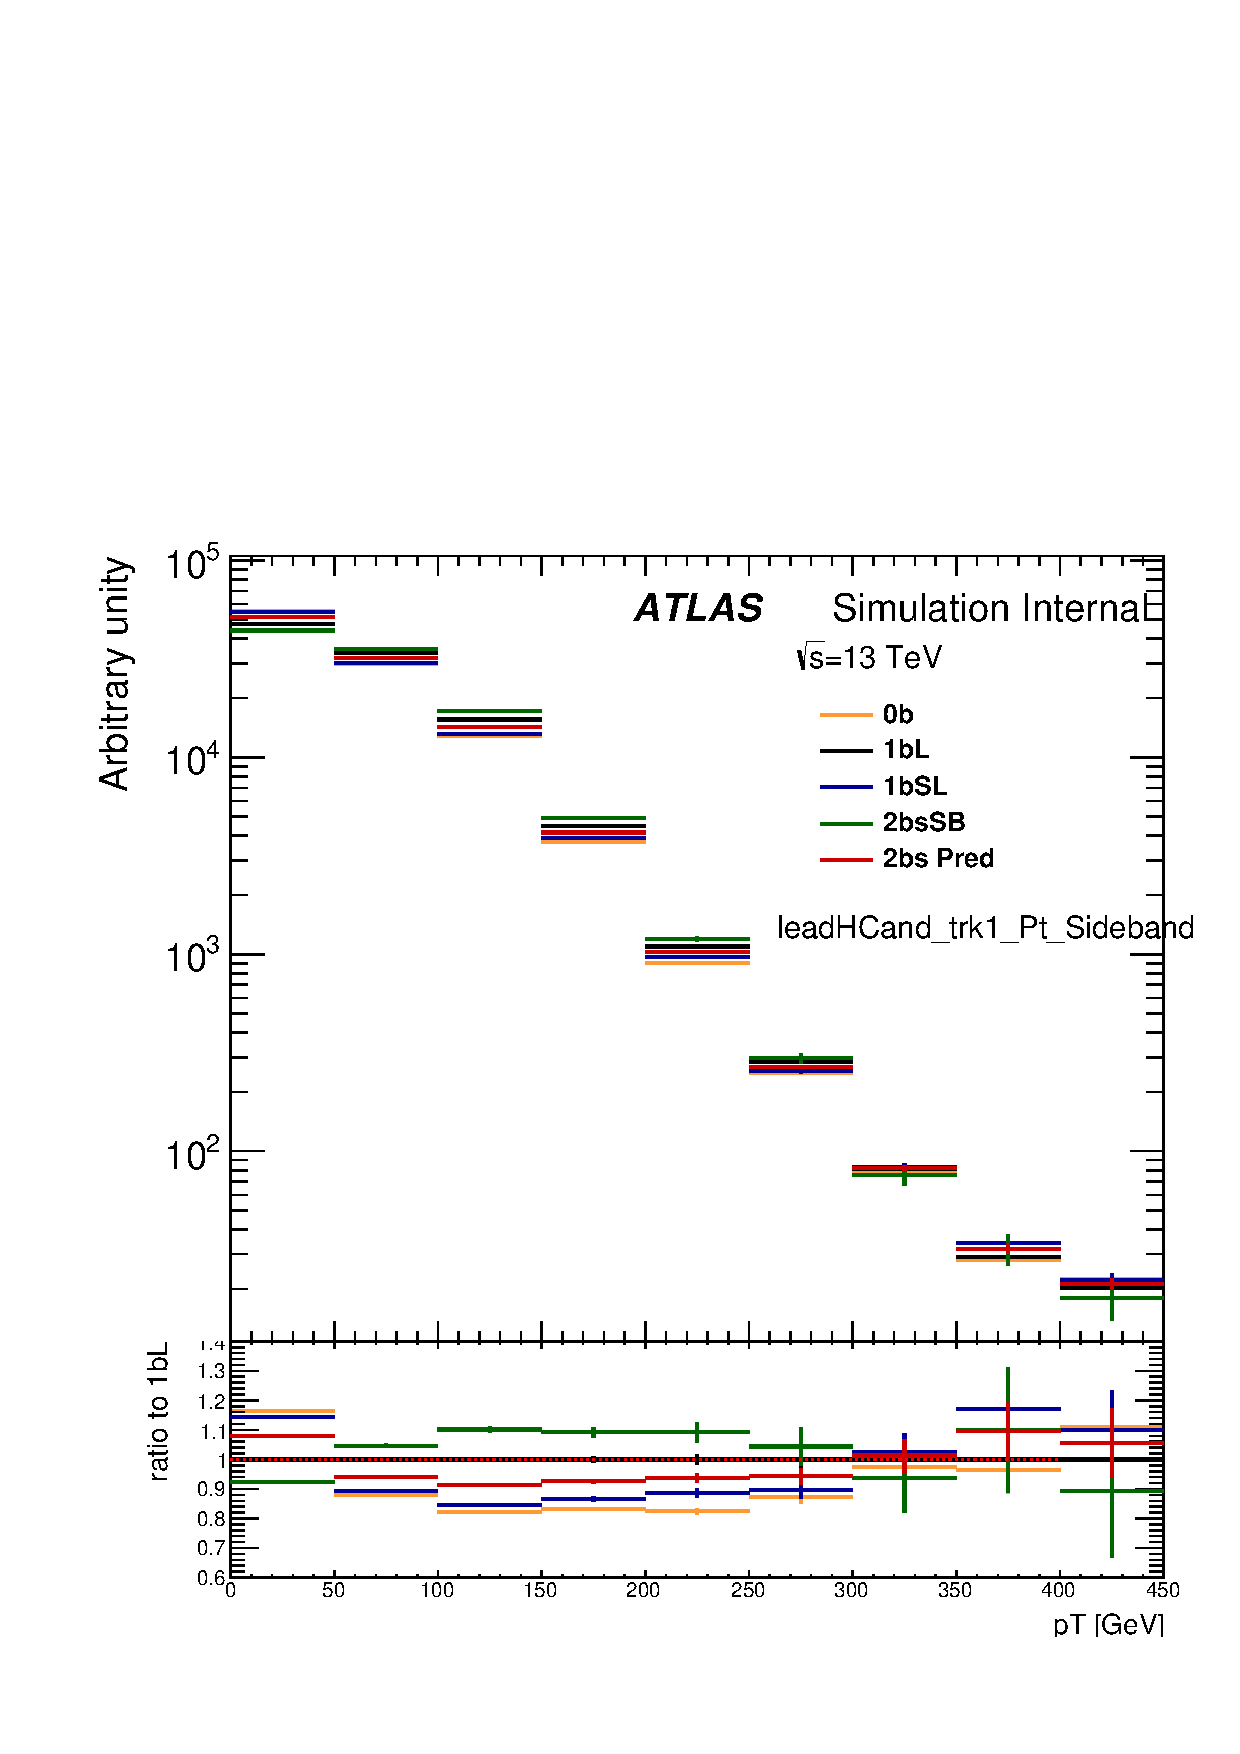
\includegraphics[width=0.25\textwidth,angle=-90]{figures/boosted/AppendixDijetMC/leadHCand_trk1_Pt_Sidebanddata_log.pdf}\\
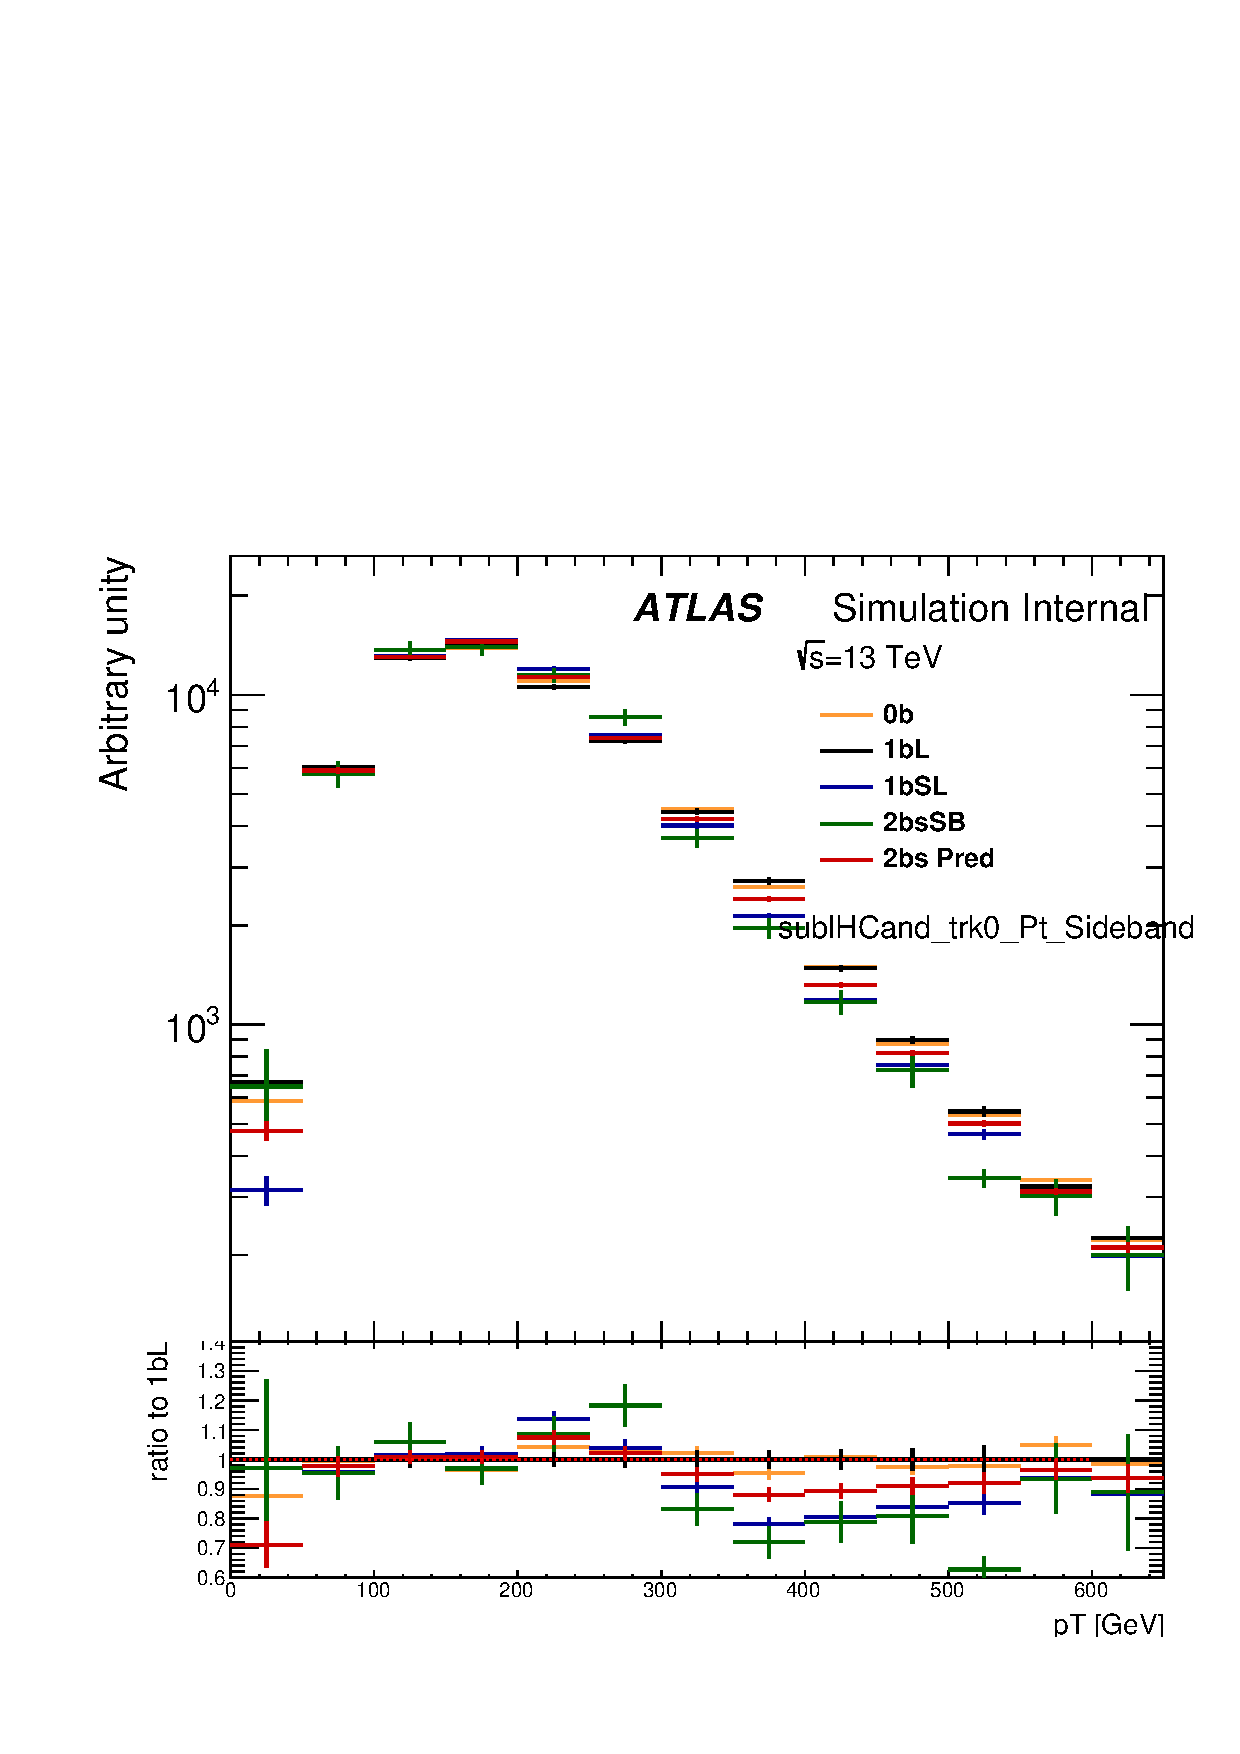
\includegraphics[width=0.25\textwidth,angle=-90]{figures/boosted/AppendixDijetMC/sublHCand_trk0_Pt_Sidebandlessbin_log.pdf}
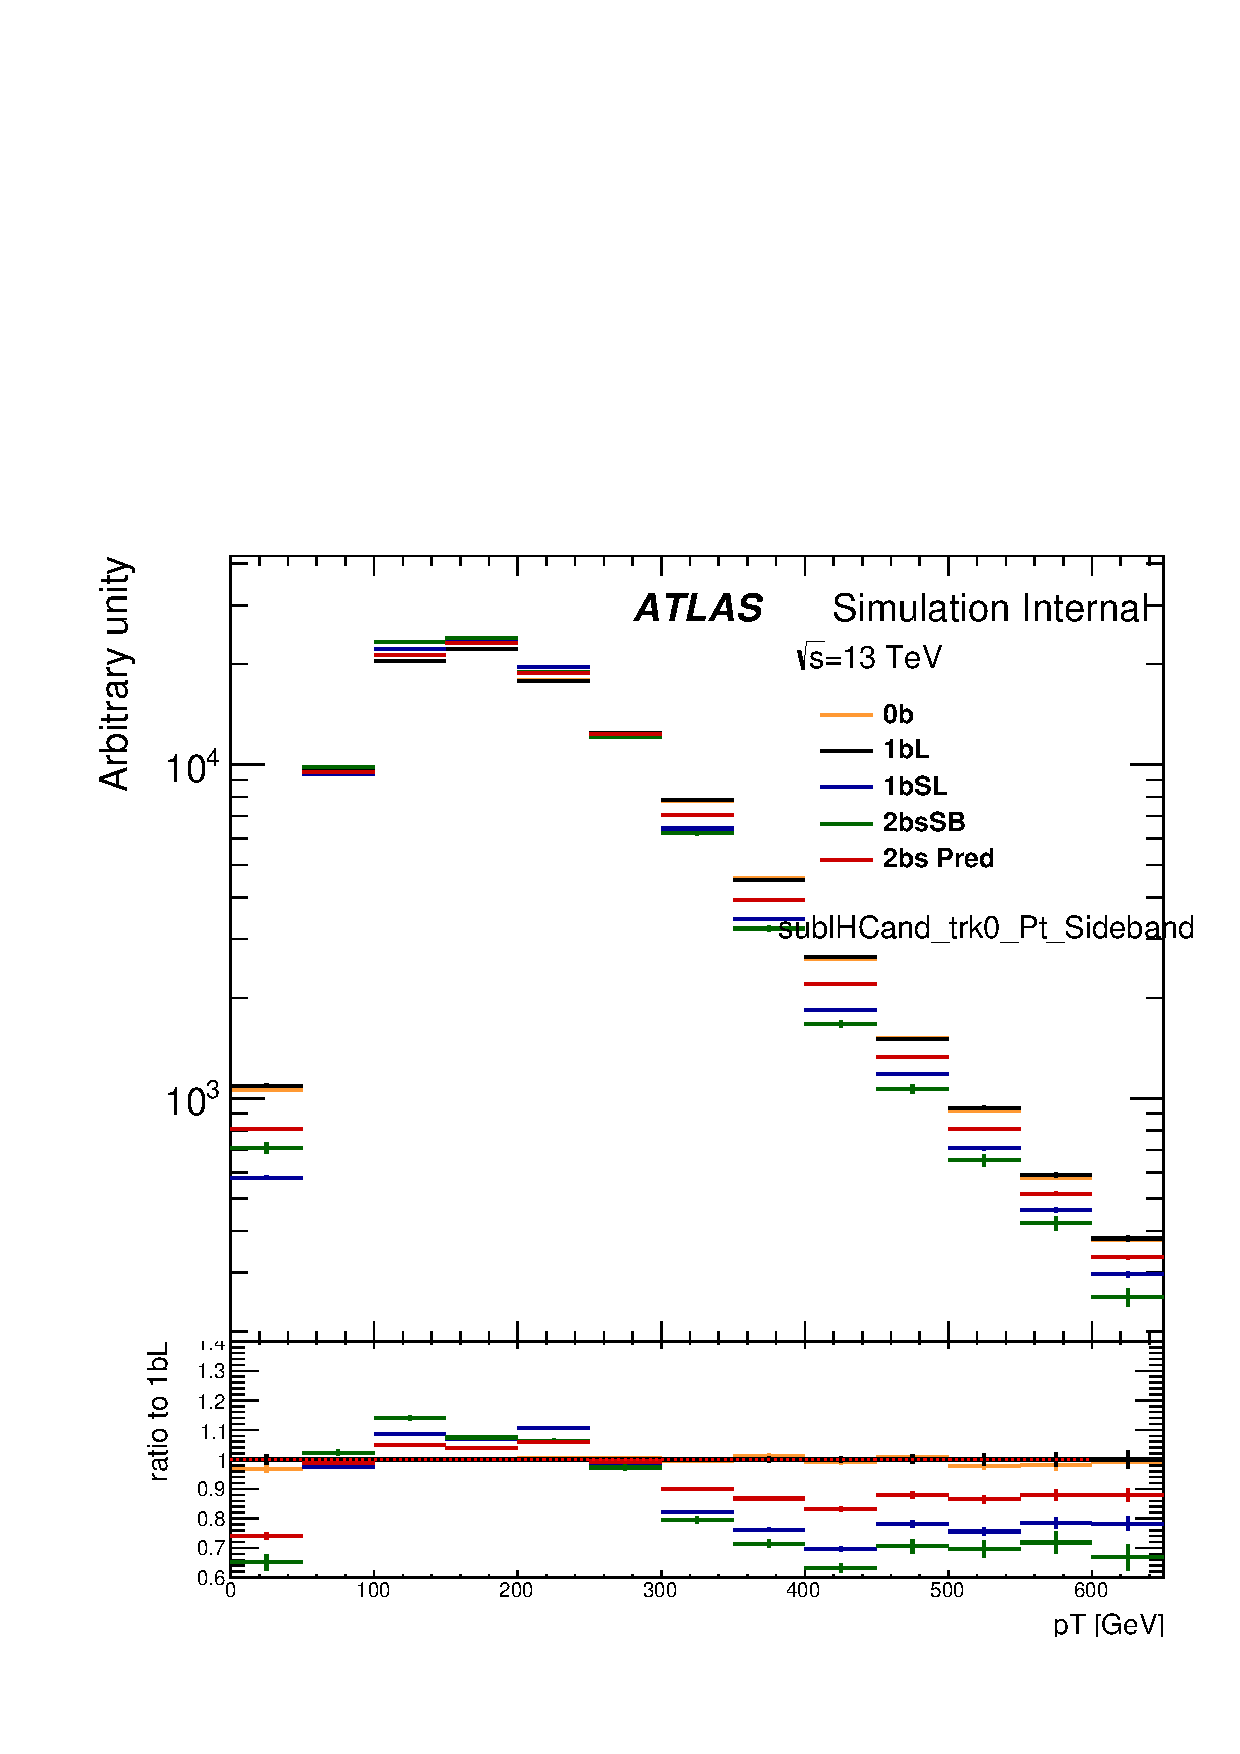
\includegraphics[width=0.25\textwidth,angle=-90]{figures/boosted/AppendixDijetMC/sublHCand_trk0_Pt_Sidebanddata_log.pdf}\\
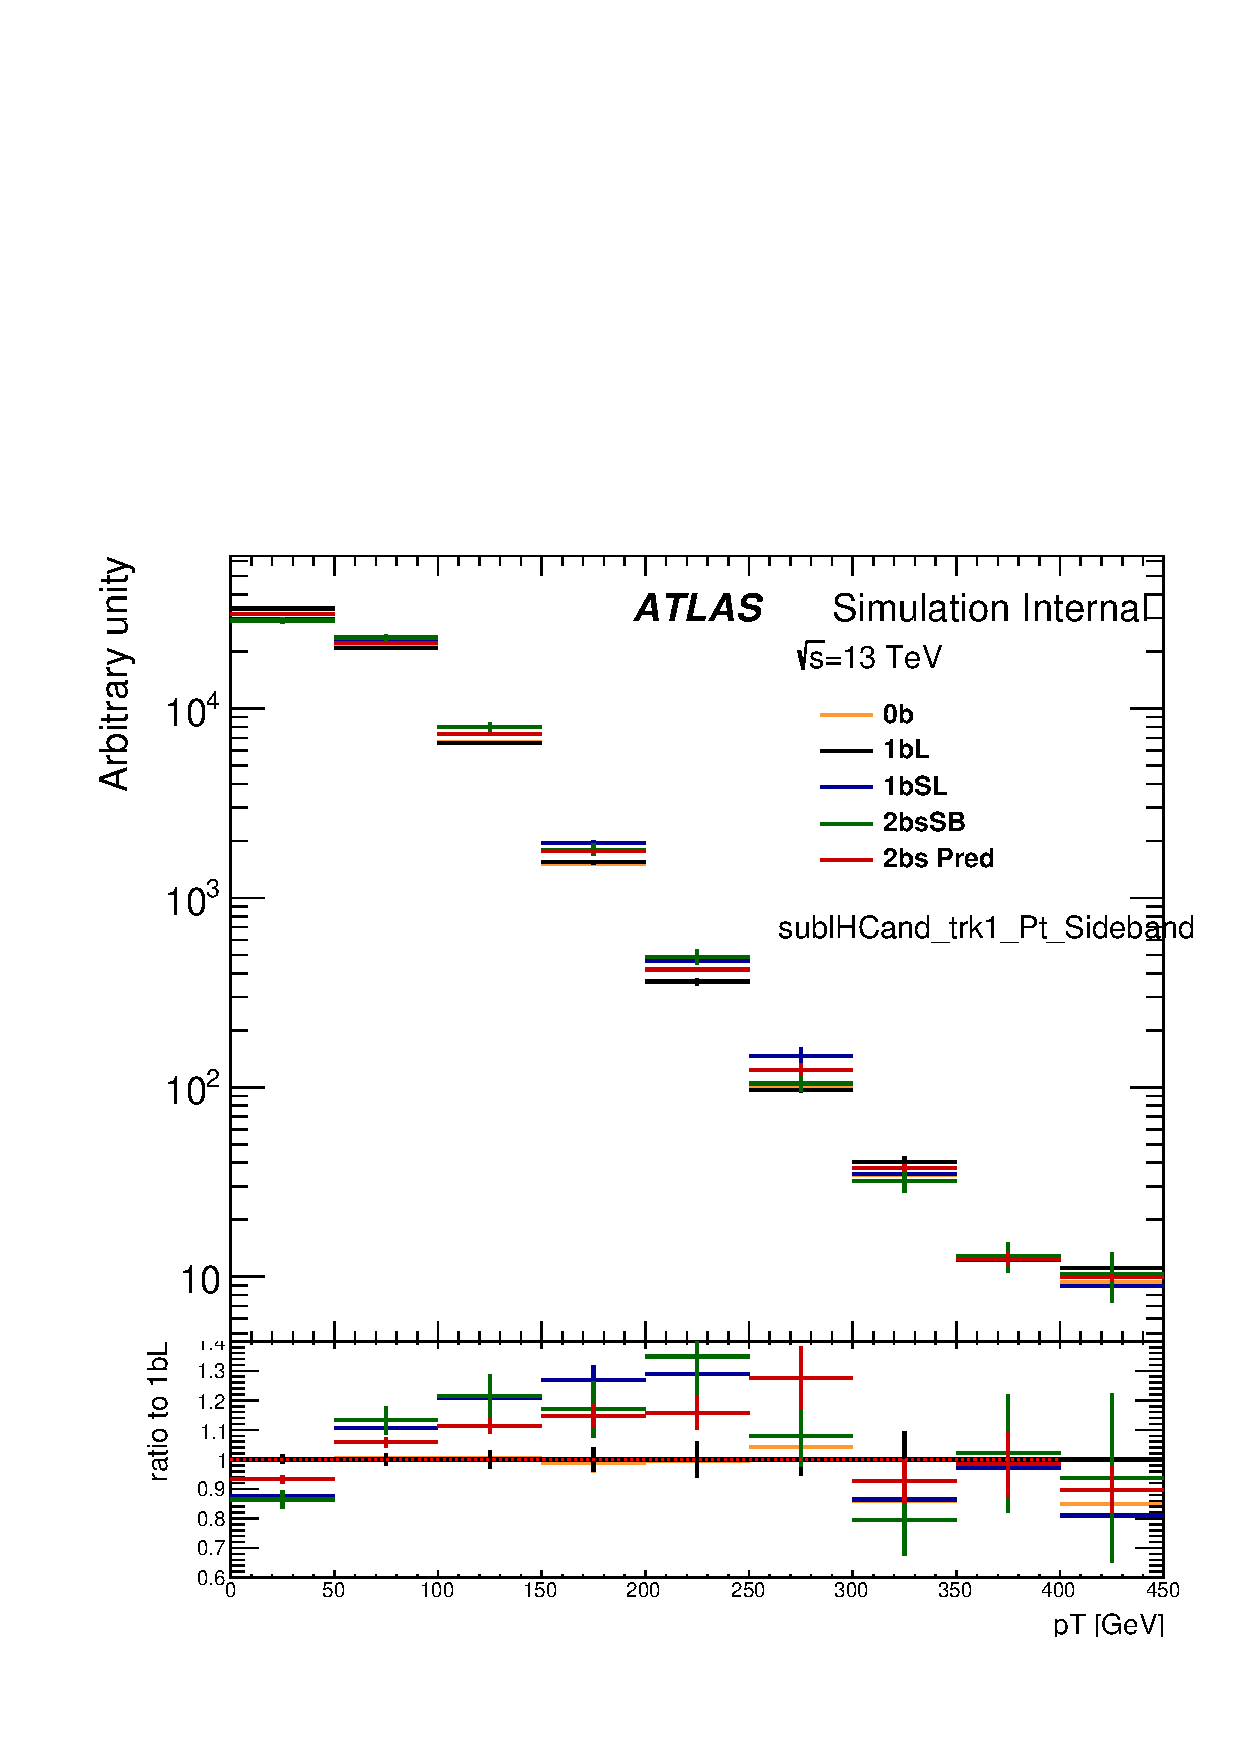
\includegraphics[width=0.25\textwidth,angle=-90]{figures/boosted/AppendixDijetMC/sublHCand_trk1_Pt_Sidebandlessbin_log.pdf}
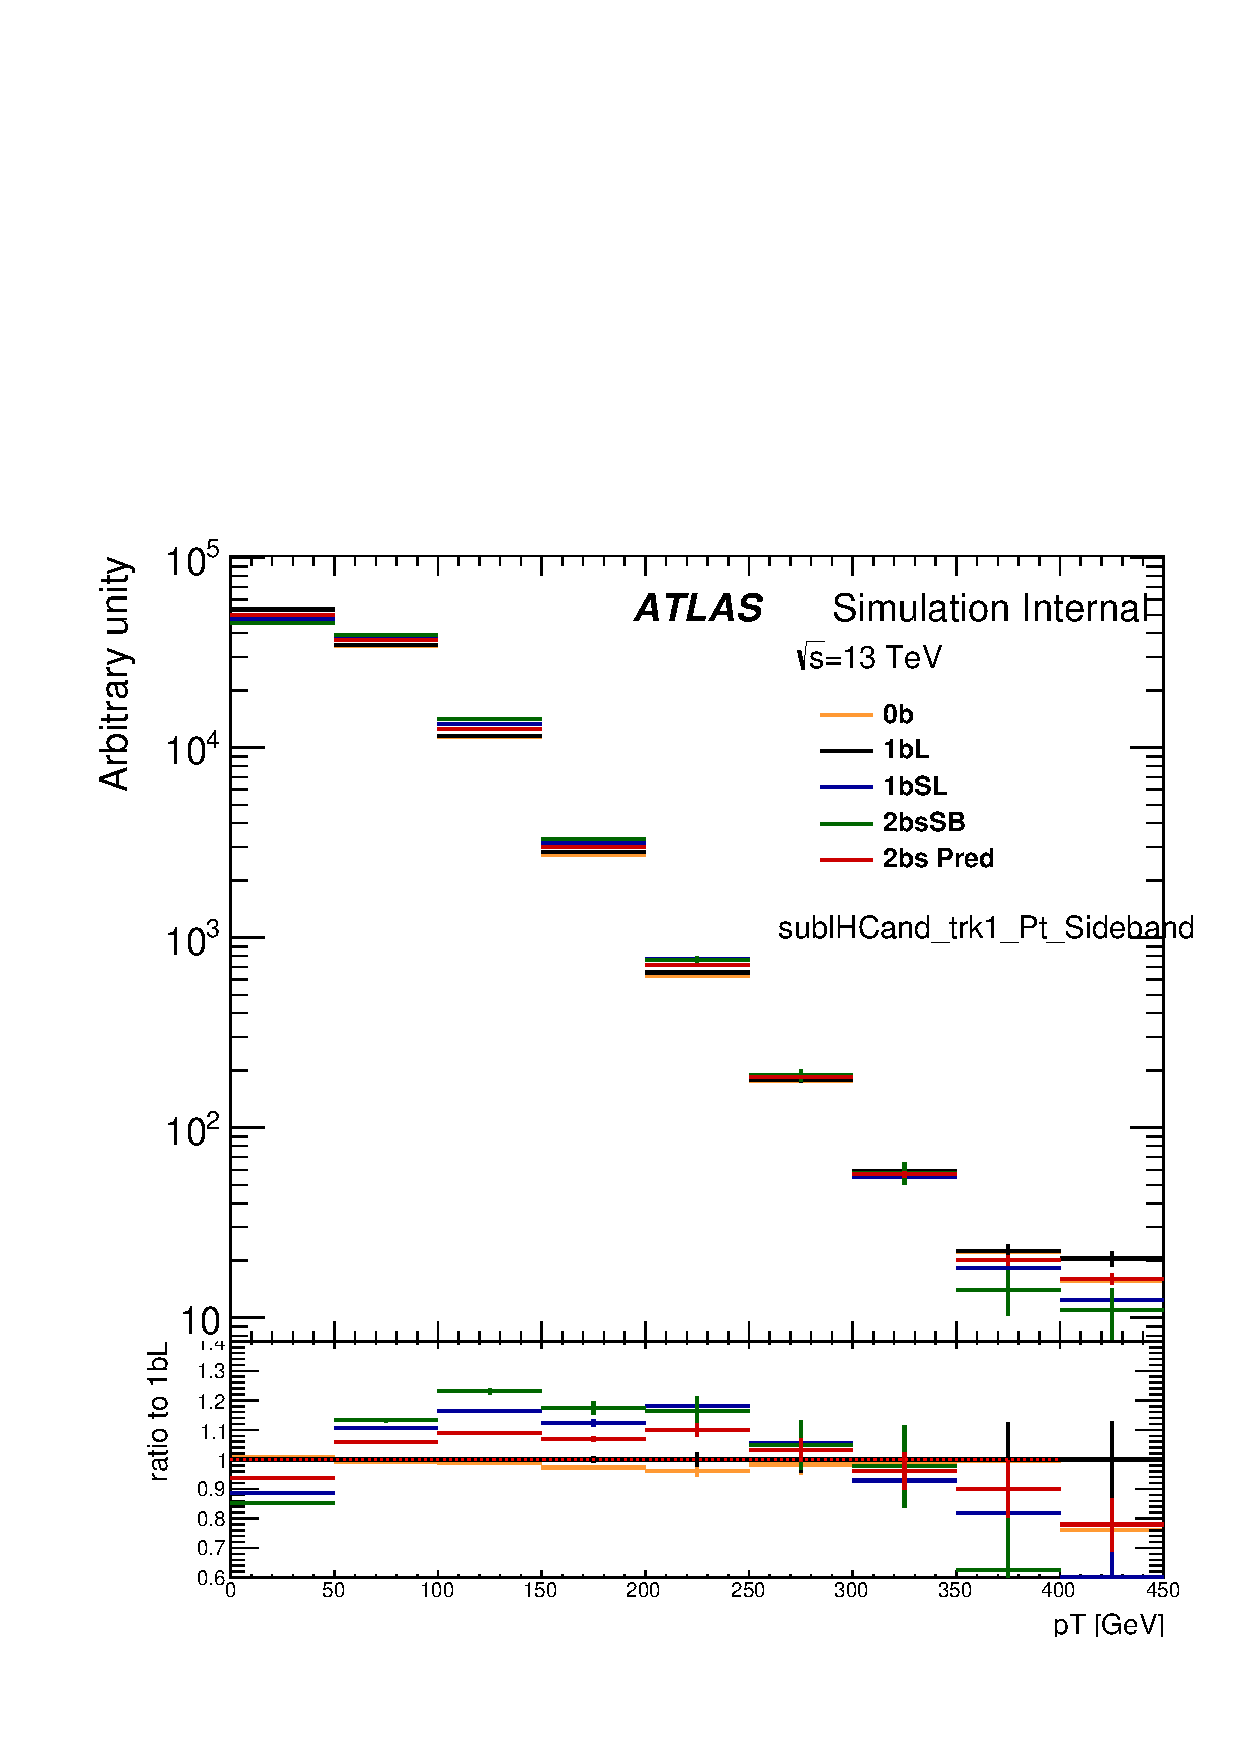
\includegraphics[width=0.25\textwidth,angle=-90]{figures/boosted/AppendixDijetMC/sublHCand_trk1_Pt_Sidebanddata_log.pdf}

 \caption{Track jet $p_{T}$ distributions together with the 2bs prediction as a comparison for the dijet MC (left) and the data (right). (First row) Leading track jet on leading Higgs candidate, (second row) subleading track jet on leading Higgs candidate, (third row) leading track jet on subleading Higgs candidate and (fourth row) subleading track jet on subleading Higgs candidate have been shown for the different regions as described in the text. All distributions are normalised according to the 2bs region.}

\label{fig:TjPred}
\end{center}
\end{figure*}

